% Created by tikzDevice version 0.12.3.1 on 2021-12-13 18:42:18
% !TEX encoding = UTF-8 Unicode
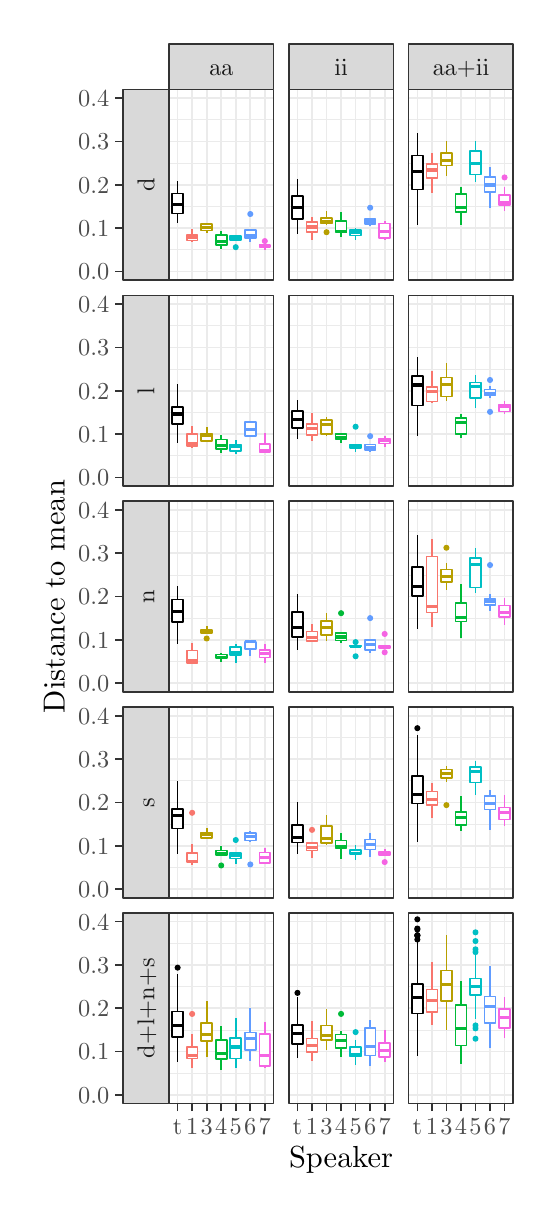
\begin{tikzpicture}[x=1pt,y=1pt]
\definecolor{fillColor}{RGB}{255,255,255}
\begin{scope}
\definecolor{drawColor}{RGB}{255,255,255}
\definecolor{fillColor}{RGB}{255,255,255}

\path[draw=drawColor,line width= 0.6pt,line join=round,line cap=round,fill=fillColor] ( -0.00,  0.00) rectangle (180.67,419.17);
\end{scope}
\begin{scope}
\definecolor{fillColor}{RGB}{255,255,255}

\path[fill=fillColor] ( 50.73,328.21) rectangle ( 88.54,397.09);
\definecolor{drawColor}{gray}{0.92}

\path[draw=drawColor,line width= 0.3pt,line join=round] ( 50.73,339.17) --
	( 88.54,339.17);

\path[draw=drawColor,line width= 0.3pt,line join=round] ( 50.73,354.83) --
	( 88.54,354.83);

\path[draw=drawColor,line width= 0.3pt,line join=round] ( 50.73,370.48) --
	( 88.54,370.48);

\path[draw=drawColor,line width= 0.3pt,line join=round] ( 50.73,386.14) --
	( 88.54,386.14);

\path[draw=drawColor,line width= 0.6pt,line join=round] ( 50.73,331.34) --
	( 88.54,331.34);

\path[draw=drawColor,line width= 0.6pt,line join=round] ( 50.73,347.00) --
	( 88.54,347.00);

\path[draw=drawColor,line width= 0.6pt,line join=round] ( 50.73,362.65) --
	( 88.54,362.65);

\path[draw=drawColor,line width= 0.6pt,line join=round] ( 50.73,378.31) --
	( 88.54,378.31);

\path[draw=drawColor,line width= 0.6pt,line join=round] ( 50.73,393.96) --
	( 88.54,393.96);

\path[draw=drawColor,line width= 0.6pt,line join=round] ( 53.88,328.21) --
	( 53.88,397.09);

\path[draw=drawColor,line width= 0.6pt,line join=round] ( 59.13,328.21) --
	( 59.13,397.09);

\path[draw=drawColor,line width= 0.6pt,line join=round] ( 64.38,328.21) --
	( 64.38,397.09);

\path[draw=drawColor,line width= 0.6pt,line join=round] ( 69.64,328.21) --
	( 69.64,397.09);

\path[draw=drawColor,line width= 0.6pt,line join=round] ( 74.89,328.21) --
	( 74.89,397.09);

\path[draw=drawColor,line width= 0.6pt,line join=round] ( 80.14,328.21) --
	( 80.14,397.09);

\path[draw=drawColor,line width= 0.6pt,line join=round] ( 85.39,328.21) --
	( 85.39,397.09);
\definecolor{drawColor}{RGB}{248,118,109}

\path[draw=drawColor,line width= 0.6pt,line join=round] ( 59.13,344.66) -- ( 59.13,346.61);

\path[draw=drawColor,line width= 0.6pt,line join=round] ( 59.13,342.58) -- ( 59.13,341.91);

\path[draw=drawColor,line width= 0.6pt,line join=round,line cap=round,fill=fillColor] ( 57.16,344.66) --
	( 57.16,342.58) --
	( 61.10,342.58) --
	( 61.10,344.66) --
	( 57.16,344.66) --
	cycle;

\path[draw=drawColor,line width= 1.1pt,line join=round] ( 57.16,343.58) -- ( 61.10,343.58);
\definecolor{drawColor}{RGB}{183,159,0}

\path[draw=drawColor,line width= 0.6pt,line join=round] ( 64.38,348.53) -- ( 64.38,348.81);

\path[draw=drawColor,line width= 0.6pt,line join=round] ( 64.38,346.16) -- ( 64.38,345.25);

\path[draw=drawColor,line width= 0.6pt,line join=round,line cap=round,fill=fillColor] ( 62.41,348.53) --
	( 62.41,346.16) --
	( 66.35,346.16) --
	( 66.35,348.53) --
	( 62.41,348.53) --
	cycle;

\path[draw=drawColor,line width= 1.1pt,line join=round] ( 62.41,347.18) -- ( 66.35,347.18);
\definecolor{drawColor}{RGB}{0,186,56}

\path[draw=drawColor,line width= 0.6pt,line join=round] ( 69.64,344.56) -- ( 69.64,346.10);

\path[draw=drawColor,line width= 0.6pt,line join=round] ( 69.64,340.92) -- ( 69.64,339.50);

\path[draw=drawColor,line width= 0.6pt,line join=round,line cap=round,fill=fillColor] ( 67.67,344.56) --
	( 67.67,340.92) --
	( 71.61,340.92) --
	( 71.61,344.56) --
	( 67.67,344.56) --
	cycle;

\path[draw=drawColor,line width= 1.1pt,line join=round] ( 67.67,342.26) -- ( 71.61,342.26);
\definecolor{drawColor}{RGB}{0,191,196}
\definecolor{fillColor}{RGB}{0,191,196}

\path[draw=drawColor,line width= 0.4pt,line join=round,line cap=round,fill=fillColor] ( 74.89,340.15) circle (  0.89);

\path[draw=drawColor,line width= 0.6pt,line join=round] ( 74.89,344.09) -- ( 74.89,344.67);

\path[draw=drawColor,line width= 0.6pt,line join=round] ( 74.89,342.84) -- ( 74.89,342.82);
\definecolor{fillColor}{RGB}{255,255,255}

\path[draw=drawColor,line width= 0.6pt,line join=round,line cap=round,fill=fillColor] ( 72.92,344.09) --
	( 72.92,342.84) --
	( 76.86,342.84) --
	( 76.86,344.09) --
	( 72.92,344.09) --
	cycle;

\path[draw=drawColor,line width= 1.1pt,line join=round] ( 72.92,343.13) -- ( 76.86,343.13);
\definecolor{drawColor}{RGB}{97,156,255}
\definecolor{fillColor}{RGB}{97,156,255}

\path[draw=drawColor,line width= 0.4pt,line join=round,line cap=round,fill=fillColor] ( 80.14,352.13) circle (  0.89);

\path[draw=drawColor,line width= 0.6pt,line join=round] ( 80.14,346.37) -- ( 80.14,346.85);

\path[draw=drawColor,line width= 0.6pt,line join=round] ( 80.14,343.51) -- ( 80.14,342.14);
\definecolor{fillColor}{RGB}{255,255,255}

\path[draw=drawColor,line width= 0.6pt,line join=round,line cap=round,fill=fillColor] ( 78.17,346.37) --
	( 78.17,343.51) --
	( 82.11,343.51) --
	( 82.11,346.37) --
	( 78.17,346.37) --
	cycle;

\path[draw=drawColor,line width= 1.1pt,line join=round] ( 78.17,344.39) -- ( 82.11,344.39);
\definecolor{drawColor}{RGB}{245,100,227}
\definecolor{fillColor}{RGB}{245,100,227}

\path[draw=drawColor,line width= 0.4pt,line join=round,line cap=round,fill=fillColor] ( 85.39,342.35) circle (  0.89);

\path[draw=drawColor,line width= 0.6pt,line join=round] ( 85.39,340.95) -- ( 85.39,341.02);

\path[draw=drawColor,line width= 0.6pt,line join=round] ( 85.39,340.13) -- ( 85.39,339.00);
\definecolor{fillColor}{RGB}{255,255,255}

\path[draw=drawColor,line width= 0.6pt,line join=round,line cap=round,fill=fillColor] ( 83.42,340.95) --
	( 83.42,340.13) --
	( 87.36,340.13) --
	( 87.36,340.95) --
	( 83.42,340.95) --
	cycle;

\path[draw=drawColor,line width= 1.1pt,line join=round] ( 83.42,340.64) -- ( 87.36,340.64);
\definecolor{drawColor}{RGB}{0,0,0}

\path[draw=drawColor,line width= 0.6pt,line join=round] ( 53.88,359.52) -- ( 53.88,364.04);

\path[draw=drawColor,line width= 0.6pt,line join=round] ( 53.88,352.35) -- ( 53.88,348.71);

\path[draw=drawColor,line width= 0.6pt,line join=round,line cap=round,fill=fillColor] ( 51.91,359.52) --
	( 51.91,352.35) --
	( 55.85,352.35) --
	( 55.85,359.52) --
	( 51.91,359.52) --
	cycle;

\path[draw=drawColor,line width= 1.1pt,line join=round] ( 51.91,355.73) -- ( 55.85,355.73);
\definecolor{drawColor}{gray}{0.20}

\path[draw=drawColor,line width= 0.6pt,line join=round,line cap=round] ( 50.73,328.21) rectangle ( 88.54,397.09);
\end{scope}
\begin{scope}
\definecolor{fillColor}{RGB}{255,255,255}

\path[fill=fillColor] ( 50.73,253.83) rectangle ( 88.54,322.71);
\definecolor{drawColor}{gray}{0.92}

\path[draw=drawColor,line width= 0.3pt,line join=round] ( 50.73,264.79) --
	( 88.54,264.79);

\path[draw=drawColor,line width= 0.3pt,line join=round] ( 50.73,280.44) --
	( 88.54,280.44);

\path[draw=drawColor,line width= 0.3pt,line join=round] ( 50.73,296.10) --
	( 88.54,296.10);

\path[draw=drawColor,line width= 0.3pt,line join=round] ( 50.73,311.75) --
	( 88.54,311.75);

\path[draw=drawColor,line width= 0.6pt,line join=round] ( 50.73,256.96) --
	( 88.54,256.96);

\path[draw=drawColor,line width= 0.6pt,line join=round] ( 50.73,272.62) --
	( 88.54,272.62);

\path[draw=drawColor,line width= 0.6pt,line join=round] ( 50.73,288.27) --
	( 88.54,288.27);

\path[draw=drawColor,line width= 0.6pt,line join=round] ( 50.73,303.93) --
	( 88.54,303.93);

\path[draw=drawColor,line width= 0.6pt,line join=round] ( 50.73,319.58) --
	( 88.54,319.58);

\path[draw=drawColor,line width= 0.6pt,line join=round] ( 53.88,253.83) --
	( 53.88,322.71);

\path[draw=drawColor,line width= 0.6pt,line join=round] ( 59.13,253.83) --
	( 59.13,322.71);

\path[draw=drawColor,line width= 0.6pt,line join=round] ( 64.38,253.83) --
	( 64.38,322.71);

\path[draw=drawColor,line width= 0.6pt,line join=round] ( 69.64,253.83) --
	( 69.64,322.71);

\path[draw=drawColor,line width= 0.6pt,line join=round] ( 74.89,253.83) --
	( 74.89,322.71);

\path[draw=drawColor,line width= 0.6pt,line join=round] ( 80.14,253.83) --
	( 80.14,322.71);

\path[draw=drawColor,line width= 0.6pt,line join=round] ( 85.39,253.83) --
	( 85.39,322.71);
\definecolor{drawColor}{RGB}{248,118,109}

\path[draw=drawColor,line width= 0.6pt,line join=round] ( 59.13,272.75) -- ( 59.13,275.53);

\path[draw=drawColor,line width= 0.6pt,line join=round] ( 59.13,268.39) -- ( 59.13,267.42);

\path[draw=drawColor,line width= 0.6pt,line join=round,line cap=round,fill=fillColor] ( 57.16,272.75) --
	( 57.16,268.39) --
	( 61.10,268.39) --
	( 61.10,272.75) --
	( 57.16,272.75) --
	cycle;

\path[draw=drawColor,line width= 1.1pt,line join=round] ( 57.16,269.14) -- ( 61.10,269.14);
\definecolor{drawColor}{RGB}{183,159,0}

\path[draw=drawColor,line width= 0.6pt,line join=round] ( 64.38,272.85) -- ( 64.38,275.26);

\path[draw=drawColor,line width= 0.6pt,line join=round] ( 64.38,270.02) -- ( 64.38,270.00);

\path[draw=drawColor,line width= 0.6pt,line join=round,line cap=round,fill=fillColor] ( 62.41,272.85) --
	( 62.41,270.02) --
	( 66.35,270.02) --
	( 66.35,272.85) --
	( 62.41,272.85) --
	cycle;

\path[draw=drawColor,line width= 1.1pt,line join=round] ( 62.41,272.22) -- ( 66.35,272.22);
\definecolor{drawColor}{RGB}{0,186,56}

\path[draw=drawColor,line width= 0.6pt,line join=round] ( 69.64,270.70) -- ( 69.64,272.23);

\path[draw=drawColor,line width= 0.6pt,line join=round] ( 69.64,267.24) -- ( 69.64,265.64);

\path[draw=drawColor,line width= 0.6pt,line join=round,line cap=round,fill=fillColor] ( 67.67,270.70) --
	( 67.67,267.24) --
	( 71.61,267.24) --
	( 71.61,270.70) --
	( 67.67,270.70) --
	cycle;

\path[draw=drawColor,line width= 1.1pt,line join=round] ( 67.67,268.62) -- ( 71.61,268.62);
\definecolor{drawColor}{RGB}{0,191,196}

\path[draw=drawColor,line width= 0.6pt,line join=round] ( 74.89,268.89) -- ( 74.89,270.55);

\path[draw=drawColor,line width= 0.6pt,line join=round] ( 74.89,266.44) -- ( 74.89,265.32);

\path[draw=drawColor,line width= 0.6pt,line join=round,line cap=round,fill=fillColor] ( 72.92,268.89) --
	( 72.92,266.44) --
	( 76.86,266.44) --
	( 76.86,268.89) --
	( 72.92,268.89) --
	cycle;

\path[draw=drawColor,line width= 1.1pt,line join=round] ( 72.92,268.29) -- ( 76.86,268.29);
\definecolor{drawColor}{RGB}{97,156,255}

\path[draw=drawColor,line width= 0.6pt,line join=round] ( 80.14,276.90) -- ( 80.14,277.37);

\path[draw=drawColor,line width= 0.6pt,line join=round] ( 80.14,271.91) -- ( 80.14,271.80);

\path[draw=drawColor,line width= 0.6pt,line join=round,line cap=round,fill=fillColor] ( 78.17,276.90) --
	( 78.17,271.91) --
	( 82.11,271.91) --
	( 82.11,276.90) --
	( 78.17,276.90) --
	cycle;

\path[draw=drawColor,line width= 1.1pt,line join=round] ( 78.17,274.28) -- ( 82.11,274.28);
\definecolor{drawColor}{RGB}{245,100,227}

\path[draw=drawColor,line width= 0.6pt,line join=round] ( 85.39,269.00) -- ( 85.39,272.92);

\path[draw=drawColor,line width= 0.6pt,line join=round] ( 85.39,266.02) -- ( 85.39,265.86);

\path[draw=drawColor,line width= 0.6pt,line join=round,line cap=round,fill=fillColor] ( 83.42,269.00) --
	( 83.42,266.02) --
	( 87.36,266.02) --
	( 87.36,269.00) --
	( 83.42,269.00) --
	cycle;

\path[draw=drawColor,line width= 1.1pt,line join=round] ( 83.42,266.83) -- ( 87.36,266.83);
\definecolor{drawColor}{RGB}{0,0,0}

\path[draw=drawColor,line width= 0.6pt,line join=round] ( 53.88,282.43) -- ( 53.88,290.83);

\path[draw=drawColor,line width= 0.6pt,line join=round] ( 53.88,276.32) -- ( 53.88,269.34);

\path[draw=drawColor,line width= 0.6pt,line join=round,line cap=round,fill=fillColor] ( 51.91,282.43) --
	( 51.91,276.32) --
	( 55.85,276.32) --
	( 55.85,282.43) --
	( 51.91,282.43) --
	cycle;

\path[draw=drawColor,line width= 1.1pt,line join=round] ( 51.91,279.87) -- ( 55.85,279.87);
\definecolor{drawColor}{gray}{0.20}

\path[draw=drawColor,line width= 0.6pt,line join=round,line cap=round] ( 50.73,253.83) rectangle ( 88.54,322.71);
\end{scope}
\begin{scope}
\definecolor{fillColor}{RGB}{255,255,255}

\path[fill=fillColor] ( 50.73,179.45) rectangle ( 88.54,248.33);
\definecolor{drawColor}{gray}{0.92}

\path[draw=drawColor,line width= 0.3pt,line join=round] ( 50.73,190.41) --
	( 88.54,190.41);

\path[draw=drawColor,line width= 0.3pt,line join=round] ( 50.73,206.06) --
	( 88.54,206.06);

\path[draw=drawColor,line width= 0.3pt,line join=round] ( 50.73,221.72) --
	( 88.54,221.72);

\path[draw=drawColor,line width= 0.3pt,line join=round] ( 50.73,237.37) --
	( 88.54,237.37);

\path[draw=drawColor,line width= 0.6pt,line join=round] ( 50.73,182.58) --
	( 88.54,182.58);

\path[draw=drawColor,line width= 0.6pt,line join=round] ( 50.73,198.24) --
	( 88.54,198.24);

\path[draw=drawColor,line width= 0.6pt,line join=round] ( 50.73,213.89) --
	( 88.54,213.89);

\path[draw=drawColor,line width= 0.6pt,line join=round] ( 50.73,229.55) --
	( 88.54,229.55);

\path[draw=drawColor,line width= 0.6pt,line join=round] ( 50.73,245.20) --
	( 88.54,245.20);

\path[draw=drawColor,line width= 0.6pt,line join=round] ( 53.88,179.45) --
	( 53.88,248.33);

\path[draw=drawColor,line width= 0.6pt,line join=round] ( 59.13,179.45) --
	( 59.13,248.33);

\path[draw=drawColor,line width= 0.6pt,line join=round] ( 64.38,179.45) --
	( 64.38,248.33);

\path[draw=drawColor,line width= 0.6pt,line join=round] ( 69.64,179.45) --
	( 69.64,248.33);

\path[draw=drawColor,line width= 0.6pt,line join=round] ( 74.89,179.45) --
	( 74.89,248.33);

\path[draw=drawColor,line width= 0.6pt,line join=round] ( 80.14,179.45) --
	( 80.14,248.33);

\path[draw=drawColor,line width= 0.6pt,line join=round] ( 85.39,179.45) --
	( 85.39,248.33);
\definecolor{drawColor}{RGB}{248,118,109}

\path[draw=drawColor,line width= 0.6pt,line join=round] ( 59.13,194.39) -- ( 59.13,197.00);

\path[draw=drawColor,line width= 0.6pt,line join=round] ( 59.13,189.89) -- ( 59.13,189.61);

\path[draw=drawColor,line width= 0.6pt,line join=round,line cap=round,fill=fillColor] ( 57.16,194.39) --
	( 57.16,189.89) --
	( 61.10,189.89) --
	( 61.10,194.39) --
	( 57.16,194.39) --
	cycle;

\path[draw=drawColor,line width= 1.1pt,line join=round] ( 57.16,190.68) -- ( 61.10,190.68);
\definecolor{drawColor}{RGB}{183,159,0}
\definecolor{fillColor}{RGB}{183,159,0}

\path[draw=drawColor,line width= 0.4pt,line join=round,line cap=round,fill=fillColor] ( 64.38,198.75) circle (  0.89);

\path[draw=drawColor,line width= 0.6pt,line join=round] ( 64.38,201.88) -- ( 64.38,203.36);

\path[draw=drawColor,line width= 0.6pt,line join=round] ( 64.38,200.79) -- ( 64.38,200.79);
\definecolor{fillColor}{RGB}{255,255,255}

\path[draw=drawColor,line width= 0.6pt,line join=round,line cap=round,fill=fillColor] ( 62.41,201.88) --
	( 62.41,200.79) --
	( 66.35,200.79) --
	( 66.35,201.88) --
	( 62.41,201.88) --
	cycle;

\path[draw=drawColor,line width= 1.1pt,line join=round] ( 62.41,201.79) -- ( 66.35,201.79);
\definecolor{drawColor}{RGB}{0,186,56}

\path[draw=drawColor,line width= 0.6pt,line join=round] ( 69.64,193.00) -- ( 69.64,193.60);

\path[draw=drawColor,line width= 0.6pt,line join=round] ( 69.64,191.75) -- ( 69.64,190.34);

\path[draw=drawColor,line width= 0.6pt,line join=round,line cap=round,fill=fillColor] ( 67.67,193.00) --
	( 67.67,191.75) --
	( 71.61,191.75) --
	( 71.61,193.00) --
	( 67.67,193.00) --
	cycle;

\path[draw=drawColor,line width= 1.1pt,line join=round] ( 67.67,191.92) -- ( 71.61,191.92);
\definecolor{drawColor}{RGB}{0,191,196}

\path[draw=drawColor,line width= 0.6pt,line join=round] ( 74.89,195.71) -- ( 74.89,196.65);

\path[draw=drawColor,line width= 0.6pt,line join=round] ( 74.89,192.78) -- ( 74.89,189.96);

\path[draw=drawColor,line width= 0.6pt,line join=round,line cap=round,fill=fillColor] ( 72.92,195.71) --
	( 72.92,192.78) --
	( 76.86,192.78) --
	( 76.86,195.71) --
	( 72.92,195.71) --
	cycle;

\path[draw=drawColor,line width= 1.1pt,line join=round] ( 72.92,193.57) -- ( 76.86,193.57);
\definecolor{drawColor}{RGB}{97,156,255}

\path[draw=drawColor,line width= 0.6pt,line join=round] ( 80.14,197.59) -- ( 80.14,197.99);

\path[draw=drawColor,line width= 0.6pt,line join=round] ( 80.14,194.96) -- ( 80.14,192.34);

\path[draw=drawColor,line width= 0.6pt,line join=round,line cap=round,fill=fillColor] ( 78.17,197.59) --
	( 78.17,194.96) --
	( 82.11,194.96) --
	( 82.11,197.59) --
	( 78.17,197.59) --
	cycle;

\path[draw=drawColor,line width= 1.1pt,line join=round] ( 78.17,197.50) -- ( 82.11,197.50);
\definecolor{drawColor}{RGB}{245,100,227}

\path[draw=drawColor,line width= 0.6pt,line join=round] ( 85.39,194.68) -- ( 85.39,196.59);

\path[draw=drawColor,line width= 0.6pt,line join=round] ( 85.39,191.91) -- ( 85.39,189.99);

\path[draw=drawColor,line width= 0.6pt,line join=round,line cap=round,fill=fillColor] ( 83.42,194.68) --
	( 83.42,191.91) --
	( 87.36,191.91) --
	( 87.36,194.68) --
	( 83.42,194.68) --
	cycle;

\path[draw=drawColor,line width= 1.1pt,line join=round] ( 83.42,193.16) -- ( 87.36,193.16);
\definecolor{drawColor}{RGB}{0,0,0}

\path[draw=drawColor,line width= 0.6pt,line join=round] ( 53.88,212.79) -- ( 53.88,217.65);

\path[draw=drawColor,line width= 0.6pt,line join=round] ( 53.88,204.76) -- ( 53.88,196.79);

\path[draw=drawColor,line width= 0.6pt,line join=round,line cap=round,fill=fillColor] ( 51.91,212.79) --
	( 51.91,204.76) --
	( 55.85,204.76) --
	( 55.85,212.79) --
	( 51.91,212.79) --
	cycle;

\path[draw=drawColor,line width= 1.1pt,line join=round] ( 51.91,208.33) -- ( 55.85,208.33);
\definecolor{drawColor}{gray}{0.20}

\path[draw=drawColor,line width= 0.6pt,line join=round,line cap=round] ( 50.73,179.45) rectangle ( 88.54,248.33);
\end{scope}
\begin{scope}
\definecolor{fillColor}{RGB}{255,255,255}

\path[fill=fillColor] ( 50.73,105.07) rectangle ( 88.54,173.95);
\definecolor{drawColor}{gray}{0.92}

\path[draw=drawColor,line width= 0.3pt,line join=round] ( 50.73,116.03) --
	( 88.54,116.03);

\path[draw=drawColor,line width= 0.3pt,line join=round] ( 50.73,131.68) --
	( 88.54,131.68);

\path[draw=drawColor,line width= 0.3pt,line join=round] ( 50.73,147.34) --
	( 88.54,147.34);

\path[draw=drawColor,line width= 0.3pt,line join=round] ( 50.73,162.99) --
	( 88.54,162.99);

\path[draw=drawColor,line width= 0.6pt,line join=round] ( 50.73,108.20) --
	( 88.54,108.20);

\path[draw=drawColor,line width= 0.6pt,line join=round] ( 50.73,123.85) --
	( 88.54,123.85);

\path[draw=drawColor,line width= 0.6pt,line join=round] ( 50.73,139.51) --
	( 88.54,139.51);

\path[draw=drawColor,line width= 0.6pt,line join=round] ( 50.73,155.16) --
	( 88.54,155.16);

\path[draw=drawColor,line width= 0.6pt,line join=round] ( 50.73,170.82) --
	( 88.54,170.82);

\path[draw=drawColor,line width= 0.6pt,line join=round] ( 53.88,105.07) --
	( 53.88,173.95);

\path[draw=drawColor,line width= 0.6pt,line join=round] ( 59.13,105.07) --
	( 59.13,173.95);

\path[draw=drawColor,line width= 0.6pt,line join=round] ( 64.38,105.07) --
	( 64.38,173.95);

\path[draw=drawColor,line width= 0.6pt,line join=round] ( 69.64,105.07) --
	( 69.64,173.95);

\path[draw=drawColor,line width= 0.6pt,line join=round] ( 74.89,105.07) --
	( 74.89,173.95);

\path[draw=drawColor,line width= 0.6pt,line join=round] ( 80.14,105.07) --
	( 80.14,173.95);

\path[draw=drawColor,line width= 0.6pt,line join=round] ( 85.39,105.07) --
	( 85.39,173.95);
\definecolor{drawColor}{RGB}{248,118,109}
\definecolor{fillColor}{RGB}{248,118,109}

\path[draw=drawColor,line width= 0.4pt,line join=round,line cap=round,fill=fillColor] ( 59.13,135.77) circle (  0.89);

\path[draw=drawColor,line width= 0.6pt,line join=round] ( 59.13,121.24) -- ( 59.13,124.47);

\path[draw=drawColor,line width= 0.6pt,line join=round] ( 59.13,117.87) -- ( 59.13,116.77);
\definecolor{fillColor}{RGB}{255,255,255}

\path[draw=drawColor,line width= 0.6pt,line join=round,line cap=round,fill=fillColor] ( 57.16,121.24) --
	( 57.16,117.87) --
	( 61.10,117.87) --
	( 61.10,121.24) --
	( 57.16,121.24) --
	cycle;

\path[draw=drawColor,line width= 1.1pt,line join=round] ( 57.16,118.33) -- ( 61.10,118.33);
\definecolor{drawColor}{RGB}{183,159,0}

\path[draw=drawColor,line width= 0.6pt,line join=round] ( 64.38,128.61) -- ( 64.38,130.13);

\path[draw=drawColor,line width= 0.6pt,line join=round] ( 64.38,126.63) -- ( 64.38,126.29);

\path[draw=drawColor,line width= 0.6pt,line join=round,line cap=round,fill=fillColor] ( 62.41,128.61) --
	( 62.41,126.63) --
	( 66.35,126.63) --
	( 66.35,128.61) --
	( 62.41,128.61) --
	cycle;

\path[draw=drawColor,line width= 1.1pt,line join=round] ( 62.41,127.86) -- ( 66.35,127.86);
\definecolor{drawColor}{RGB}{0,186,56}
\definecolor{fillColor}{RGB}{0,186,56}

\path[draw=drawColor,line width= 0.4pt,line join=round,line cap=round,fill=fillColor] ( 69.64,116.73) circle (  0.89);

\path[draw=drawColor,line width= 0.6pt,line join=round] ( 69.64,122.08) -- ( 69.64,123.63);

\path[draw=drawColor,line width= 0.6pt,line join=round] ( 69.64,120.41) -- ( 69.64,120.17);
\definecolor{fillColor}{RGB}{255,255,255}

\path[draw=drawColor,line width= 0.6pt,line join=round,line cap=round,fill=fillColor] ( 67.67,122.08) --
	( 67.67,120.41) --
	( 71.61,120.41) --
	( 71.61,122.08) --
	( 67.67,122.08) --
	cycle;

\path[draw=drawColor,line width= 1.1pt,line join=round] ( 67.67,121.16) -- ( 71.61,121.16);
\definecolor{drawColor}{RGB}{0,191,196}
\definecolor{fillColor}{RGB}{0,191,196}

\path[draw=drawColor,line width= 0.4pt,line join=round,line cap=round,fill=fillColor] ( 74.89,125.93) circle (  0.89);

\path[draw=drawColor,line width= 0.6pt,line join=round] ( 74.89,121.21) -- ( 74.89,121.44);

\path[draw=drawColor,line width= 0.6pt,line join=round] ( 74.89,119.20) -- ( 74.89,117.18);
\definecolor{fillColor}{RGB}{255,255,255}

\path[draw=drawColor,line width= 0.6pt,line join=round,line cap=round,fill=fillColor] ( 72.92,121.21) --
	( 72.92,119.20) --
	( 76.86,119.20) --
	( 76.86,121.21) --
	( 72.92,121.21) --
	cycle;

\path[draw=drawColor,line width= 1.1pt,line join=round] ( 72.92,120.28) -- ( 76.86,120.28);
\definecolor{drawColor}{RGB}{97,156,255}
\definecolor{fillColor}{RGB}{97,156,255}

\path[draw=drawColor,line width= 0.4pt,line join=round,line cap=round,fill=fillColor] ( 80.14,117.10) circle (  0.89);

\path[draw=drawColor,line width= 0.6pt,line join=round] ( 80.14,128.39) -- ( 80.14,129.34);

\path[draw=drawColor,line width= 0.6pt,line join=round] ( 80.14,125.74) -- ( 80.14,125.36);
\definecolor{fillColor}{RGB}{255,255,255}

\path[draw=drawColor,line width= 0.6pt,line join=round,line cap=round,fill=fillColor] ( 78.17,128.39) --
	( 78.17,125.74) --
	( 82.11,125.74) --
	( 82.11,128.39) --
	( 78.17,128.39) --
	cycle;

\path[draw=drawColor,line width= 1.1pt,line join=round] ( 78.17,127.10) -- ( 82.11,127.10);
\definecolor{drawColor}{RGB}{245,100,227}

\path[draw=drawColor,line width= 0.6pt,line join=round] ( 85.39,121.45) -- ( 85.39,123.02);

\path[draw=drawColor,line width= 0.6pt,line join=round] ( 85.39,117.59) -- ( 85.39,117.31);

\path[draw=drawColor,line width= 0.6pt,line join=round,line cap=round,fill=fillColor] ( 83.42,121.45) --
	( 83.42,117.59) --
	( 87.36,117.59) --
	( 87.36,121.45) --
	( 83.42,121.45) --
	cycle;

\path[draw=drawColor,line width= 1.1pt,line join=round] ( 83.42,119.63) -- ( 87.36,119.63);
\definecolor{drawColor}{RGB}{0,0,0}

\path[draw=drawColor,line width= 0.6pt,line join=round] ( 53.88,137.08) -- ( 53.88,147.37);

\path[draw=drawColor,line width= 0.6pt,line join=round] ( 53.88,130.04) -- ( 53.88,120.73);

\path[draw=drawColor,line width= 0.6pt,line join=round,line cap=round,fill=fillColor] ( 51.91,137.08) --
	( 51.91,130.04) --
	( 55.85,130.04) --
	( 55.85,137.08) --
	( 51.91,137.08) --
	cycle;

\path[draw=drawColor,line width= 1.1pt,line join=round] ( 51.91,134.84) -- ( 55.85,134.84);
\definecolor{drawColor}{gray}{0.20}

\path[draw=drawColor,line width= 0.6pt,line join=round,line cap=round] ( 50.73,105.07) rectangle ( 88.54,173.95);
\end{scope}
\begin{scope}
\definecolor{fillColor}{RGB}{255,255,255}

\path[fill=fillColor] ( 50.73, 30.69) rectangle ( 88.54, 99.57);
\definecolor{drawColor}{gray}{0.92}

\path[draw=drawColor,line width= 0.3pt,line join=round] ( 50.73, 41.64) --
	( 88.54, 41.64);

\path[draw=drawColor,line width= 0.3pt,line join=round] ( 50.73, 57.30) --
	( 88.54, 57.30);

\path[draw=drawColor,line width= 0.3pt,line join=round] ( 50.73, 72.95) --
	( 88.54, 72.95);

\path[draw=drawColor,line width= 0.3pt,line join=round] ( 50.73, 88.61) --
	( 88.54, 88.61);

\path[draw=drawColor,line width= 0.6pt,line join=round] ( 50.73, 33.82) --
	( 88.54, 33.82);

\path[draw=drawColor,line width= 0.6pt,line join=round] ( 50.73, 49.47) --
	( 88.54, 49.47);

\path[draw=drawColor,line width= 0.6pt,line join=round] ( 50.73, 65.13) --
	( 88.54, 65.13);

\path[draw=drawColor,line width= 0.6pt,line join=round] ( 50.73, 80.78) --
	( 88.54, 80.78);

\path[draw=drawColor,line width= 0.6pt,line join=round] ( 50.73, 96.44) --
	( 88.54, 96.44);

\path[draw=drawColor,line width= 0.6pt,line join=round] ( 53.88, 30.69) --
	( 53.88, 99.57);

\path[draw=drawColor,line width= 0.6pt,line join=round] ( 59.13, 30.69) --
	( 59.13, 99.57);

\path[draw=drawColor,line width= 0.6pt,line join=round] ( 64.38, 30.69) --
	( 64.38, 99.57);

\path[draw=drawColor,line width= 0.6pt,line join=round] ( 69.64, 30.69) --
	( 69.64, 99.57);

\path[draw=drawColor,line width= 0.6pt,line join=round] ( 74.89, 30.69) --
	( 74.89, 99.57);

\path[draw=drawColor,line width= 0.6pt,line join=round] ( 80.14, 30.69) --
	( 80.14, 99.57);

\path[draw=drawColor,line width= 0.6pt,line join=round] ( 85.39, 30.69) --
	( 85.39, 99.57);
\definecolor{drawColor}{RGB}{248,118,109}
\definecolor{fillColor}{RGB}{248,118,109}

\path[draw=drawColor,line width= 0.4pt,line join=round,line cap=round,fill=fillColor] ( 59.13, 63.09) circle (  0.89);

\path[draw=drawColor,line width= 0.6pt,line join=round] ( 59.13, 51.09) -- ( 59.13, 55.94);

\path[draw=drawColor,line width= 0.6pt,line join=round] ( 59.13, 46.96) -- ( 59.13, 43.61);
\definecolor{fillColor}{RGB}{255,255,255}

\path[draw=drawColor,line width= 0.6pt,line join=round,line cap=round,fill=fillColor] ( 57.16, 51.09) --
	( 57.16, 46.96) --
	( 61.10, 46.96) --
	( 61.10, 51.09) --
	( 57.16, 51.09) --
	cycle;

\path[draw=drawColor,line width= 1.1pt,line join=round] ( 57.16, 48.14) -- ( 61.10, 48.14);
\definecolor{drawColor}{RGB}{183,159,0}

\path[draw=drawColor,line width= 0.6pt,line join=round] ( 64.38, 59.71) -- ( 64.38, 67.58);

\path[draw=drawColor,line width= 0.6pt,line join=round] ( 64.38, 53.26) -- ( 64.38, 47.61);

\path[draw=drawColor,line width= 0.6pt,line join=round,line cap=round,fill=fillColor] ( 62.41, 59.71) --
	( 62.41, 53.26) --
	( 66.35, 53.26) --
	( 66.35, 59.71) --
	( 62.41, 59.71) --
	cycle;

\path[draw=drawColor,line width= 1.1pt,line join=round] ( 62.41, 55.48) -- ( 66.35, 55.48);
\definecolor{drawColor}{RGB}{0,186,56}

\path[draw=drawColor,line width= 0.6pt,line join=round] ( 69.64, 53.63) -- ( 69.64, 58.56);

\path[draw=drawColor,line width= 0.6pt,line join=round] ( 69.64, 46.78) -- ( 69.64, 42.73);

\path[draw=drawColor,line width= 0.6pt,line join=round,line cap=round,fill=fillColor] ( 67.67, 53.63) --
	( 67.67, 46.78) --
	( 71.61, 46.78) --
	( 71.61, 53.63) --
	( 67.67, 53.63) --
	cycle;

\path[draw=drawColor,line width= 1.1pt,line join=round] ( 67.67, 48.80) -- ( 71.61, 48.80);
\definecolor{drawColor}{RGB}{0,191,196}

\path[draw=drawColor,line width= 0.6pt,line join=round] ( 74.89, 54.36) -- ( 74.89, 61.67);

\path[draw=drawColor,line width= 0.6pt,line join=round] ( 74.89, 46.95) -- ( 74.89, 43.67);

\path[draw=drawColor,line width= 0.6pt,line join=round,line cap=round,fill=fillColor] ( 72.92, 54.36) --
	( 72.92, 46.95) --
	( 76.86, 46.95) --
	( 76.86, 54.36) --
	( 72.92, 54.36) --
	cycle;

\path[draw=drawColor,line width= 1.1pt,line join=round] ( 72.92, 51.13) -- ( 76.86, 51.13);
\definecolor{drawColor}{RGB}{97,156,255}

\path[draw=drawColor,line width= 0.6pt,line join=round] ( 80.14, 56.41) -- ( 80.14, 65.30);

\path[draw=drawColor,line width= 0.6pt,line join=round] ( 80.14, 50.01) -- ( 80.14, 46.07);

\path[draw=drawColor,line width= 0.6pt,line join=round,line cap=round,fill=fillColor] ( 78.17, 56.41) --
	( 78.17, 50.01) --
	( 82.11, 50.01) --
	( 82.11, 56.41) --
	( 78.17, 56.41) --
	cycle;

\path[draw=drawColor,line width= 1.1pt,line join=round] ( 78.17, 54.08) -- ( 82.11, 54.08);
\definecolor{drawColor}{RGB}{245,100,227}

\path[draw=drawColor,line width= 0.6pt,line join=round] ( 85.39, 55.78) -- ( 85.39, 60.25);

\path[draw=drawColor,line width= 0.6pt,line join=round] ( 85.39, 44.36) -- ( 85.39, 43.54);

\path[draw=drawColor,line width= 0.6pt,line join=round,line cap=round,fill=fillColor] ( 83.42, 55.78) --
	( 83.42, 44.36) --
	( 87.36, 44.36) --
	( 87.36, 55.78) --
	( 83.42, 55.78) --
	cycle;

\path[draw=drawColor,line width= 1.1pt,line join=round] ( 83.42, 48.15) -- ( 87.36, 48.15);
\definecolor{drawColor}{RGB}{0,0,0}
\definecolor{fillColor}{RGB}{0,0,0}

\path[draw=drawColor,line width= 0.4pt,line join=round,line cap=round,fill=fillColor] ( 53.88, 79.81) circle (  0.89);

\path[draw=drawColor,line width= 0.6pt,line join=round] ( 53.88, 63.94) -- ( 53.88, 77.34);

\path[draw=drawColor,line width= 0.6pt,line join=round] ( 53.88, 54.82) -- ( 53.88, 45.73);
\definecolor{fillColor}{RGB}{255,255,255}

\path[draw=drawColor,line width= 0.6pt,line join=round,line cap=round,fill=fillColor] ( 51.91, 63.94) --
	( 51.91, 54.82) --
	( 55.85, 54.82) --
	( 55.85, 63.94) --
	( 51.91, 63.94) --
	cycle;

\path[draw=drawColor,line width= 1.1pt,line join=round] ( 51.91, 58.80) -- ( 55.85, 58.80);
\definecolor{drawColor}{gray}{0.20}

\path[draw=drawColor,line width= 0.6pt,line join=round,line cap=round] ( 50.73, 30.69) rectangle ( 88.54, 99.57);
\end{scope}
\begin{scope}
\definecolor{fillColor}{RGB}{255,255,255}

\path[fill=fillColor] ( 94.04,328.21) rectangle (131.86,397.09);
\definecolor{drawColor}{gray}{0.92}

\path[draw=drawColor,line width= 0.3pt,line join=round] ( 94.04,339.17) --
	(131.86,339.17);

\path[draw=drawColor,line width= 0.3pt,line join=round] ( 94.04,354.83) --
	(131.86,354.83);

\path[draw=drawColor,line width= 0.3pt,line join=round] ( 94.04,370.48) --
	(131.86,370.48);

\path[draw=drawColor,line width= 0.3pt,line join=round] ( 94.04,386.14) --
	(131.86,386.14);

\path[draw=drawColor,line width= 0.6pt,line join=round] ( 94.04,331.34) --
	(131.86,331.34);

\path[draw=drawColor,line width= 0.6pt,line join=round] ( 94.04,347.00) --
	(131.86,347.00);

\path[draw=drawColor,line width= 0.6pt,line join=round] ( 94.04,362.65) --
	(131.86,362.65);

\path[draw=drawColor,line width= 0.6pt,line join=round] ( 94.04,378.31) --
	(131.86,378.31);

\path[draw=drawColor,line width= 0.6pt,line join=round] ( 94.04,393.96) --
	(131.86,393.96);

\path[draw=drawColor,line width= 0.6pt,line join=round] ( 97.19,328.21) --
	( 97.19,397.09);

\path[draw=drawColor,line width= 0.6pt,line join=round] (102.45,328.21) --
	(102.45,397.09);

\path[draw=drawColor,line width= 0.6pt,line join=round] (107.70,328.21) --
	(107.70,397.09);

\path[draw=drawColor,line width= 0.6pt,line join=round] (112.95,328.21) --
	(112.95,397.09);

\path[draw=drawColor,line width= 0.6pt,line join=round] (118.20,328.21) --
	(118.20,397.09);

\path[draw=drawColor,line width= 0.6pt,line join=round] (123.46,328.21) --
	(123.46,397.09);

\path[draw=drawColor,line width= 0.6pt,line join=round] (128.71,328.21) --
	(128.71,397.09);
\definecolor{drawColor}{RGB}{248,118,109}

\path[draw=drawColor,line width= 0.6pt,line join=round] (102.45,349.34) -- (102.45,350.94);

\path[draw=drawColor,line width= 0.6pt,line join=round] (102.45,345.73) -- (102.45,342.67);

\path[draw=drawColor,line width= 0.6pt,line join=round,line cap=round,fill=fillColor] (100.48,349.34) --
	(100.48,345.73) --
	(104.42,345.73) --
	(104.42,349.34) --
	(100.48,349.34) --
	cycle;

\path[draw=drawColor,line width= 1.1pt,line join=round] (100.48,347.44) -- (104.42,347.44);
\definecolor{drawColor}{RGB}{183,159,0}
\definecolor{fillColor}{RGB}{183,159,0}

\path[draw=drawColor,line width= 0.4pt,line join=round,line cap=round,fill=fillColor] (107.70,345.56) circle (  0.89);

\path[draw=drawColor,line width= 0.6pt,line join=round] (107.70,350.63) -- (107.70,353.30);

\path[draw=drawColor,line width= 0.6pt,line join=round] (107.70,348.66) -- (107.70,348.60);
\definecolor{fillColor}{RGB}{255,255,255}

\path[draw=drawColor,line width= 0.6pt,line join=round,line cap=round,fill=fillColor] (105.73,350.63) --
	(105.73,348.66) --
	(109.67,348.66) --
	(109.67,350.63) --
	(105.73,350.63) --
	cycle;

\path[draw=drawColor,line width= 1.1pt,line join=round] (105.73,349.33) -- (109.67,349.33);
\definecolor{drawColor}{RGB}{0,186,56}

\path[draw=drawColor,line width= 0.6pt,line join=round] (112.95,349.55) -- (112.95,352.68);

\path[draw=drawColor,line width= 0.6pt,line join=round] (112.95,345.64) -- (112.95,343.77);

\path[draw=drawColor,line width= 0.6pt,line join=round,line cap=round,fill=fillColor] (110.98,349.55) --
	(110.98,345.64) --
	(114.92,345.64) --
	(114.92,349.55) --
	(110.98,349.55) --
	cycle;

\path[draw=drawColor,line width= 1.1pt,line join=round] (110.98,345.94) -- (114.92,345.94);
\definecolor{drawColor}{RGB}{0,191,196}

\path[draw=drawColor,line width= 0.6pt,line join=round] (118.20,346.46) -- (118.20,347.10);

\path[draw=drawColor,line width= 0.6pt,line join=round] (118.20,344.34) -- (118.20,342.61);

\path[draw=drawColor,line width= 0.6pt,line join=round,line cap=round,fill=fillColor] (116.23,346.46) --
	(116.23,344.34) --
	(120.17,344.34) --
	(120.17,346.46) --
	(116.23,346.46) --
	cycle;

\path[draw=drawColor,line width= 1.1pt,line join=round] (116.23,345.50) -- (120.17,345.50);
\definecolor{drawColor}{RGB}{97,156,255}
\definecolor{fillColor}{RGB}{97,156,255}

\path[draw=drawColor,line width= 0.4pt,line join=round,line cap=round,fill=fillColor] (123.46,354.40) circle (  0.89);

\path[draw=drawColor,line width= 0.6pt,line join=round] (123.46,350.32) -- (123.46,350.56);

\path[draw=drawColor,line width= 0.6pt,line join=round] (123.46,348.62) -- (123.46,347.70);
\definecolor{fillColor}{RGB}{255,255,255}

\path[draw=drawColor,line width= 0.6pt,line join=round,line cap=round,fill=fillColor] (121.49,350.32) --
	(121.49,348.62) --
	(125.43,348.62) --
	(125.43,350.32) --
	(121.49,350.32) --
	cycle;

\path[draw=drawColor,line width= 1.1pt,line join=round] (121.49,349.58) -- (125.43,349.58);
\definecolor{drawColor}{RGB}{245,100,227}

\path[draw=drawColor,line width= 0.6pt,line join=round] (128.71,348.75) -- (128.71,349.43);

\path[draw=drawColor,line width= 0.6pt,line join=round] (128.71,343.56) -- (128.71,342.66);

\path[draw=drawColor,line width= 0.6pt,line join=round,line cap=round,fill=fillColor] (126.74,348.75) --
	(126.74,343.56) --
	(130.68,343.56) --
	(130.68,348.75) --
	(126.74,348.75) --
	cycle;

\path[draw=drawColor,line width= 1.1pt,line join=round] (126.74,345.65) -- (130.68,345.65);
\definecolor{drawColor}{RGB}{0,0,0}

\path[draw=drawColor,line width= 0.6pt,line join=round] ( 97.19,358.61) -- ( 97.19,364.84);

\path[draw=drawColor,line width= 0.6pt,line join=round] ( 97.19,350.35) -- ( 97.19,344.83);

\path[draw=drawColor,line width= 0.6pt,line join=round,line cap=round,fill=fillColor] ( 95.23,358.61) --
	( 95.23,350.35) --
	( 99.16,350.35) --
	( 99.16,358.61) --
	( 95.23,358.61) --
	cycle;

\path[draw=drawColor,line width= 1.1pt,line join=round] ( 95.23,354.53) -- ( 99.16,354.53);
\definecolor{drawColor}{gray}{0.20}

\path[draw=drawColor,line width= 0.6pt,line join=round,line cap=round] ( 94.04,328.21) rectangle (131.86,397.09);
\end{scope}
\begin{scope}
\definecolor{fillColor}{RGB}{255,255,255}

\path[fill=fillColor] ( 94.04,253.83) rectangle (131.86,322.71);
\definecolor{drawColor}{gray}{0.92}

\path[draw=drawColor,line width= 0.3pt,line join=round] ( 94.04,264.79) --
	(131.86,264.79);

\path[draw=drawColor,line width= 0.3pt,line join=round] ( 94.04,280.44) --
	(131.86,280.44);

\path[draw=drawColor,line width= 0.3pt,line join=round] ( 94.04,296.10) --
	(131.86,296.10);

\path[draw=drawColor,line width= 0.3pt,line join=round] ( 94.04,311.75) --
	(131.86,311.75);

\path[draw=drawColor,line width= 0.6pt,line join=round] ( 94.04,256.96) --
	(131.86,256.96);

\path[draw=drawColor,line width= 0.6pt,line join=round] ( 94.04,272.62) --
	(131.86,272.62);

\path[draw=drawColor,line width= 0.6pt,line join=round] ( 94.04,288.27) --
	(131.86,288.27);

\path[draw=drawColor,line width= 0.6pt,line join=round] ( 94.04,303.93) --
	(131.86,303.93);

\path[draw=drawColor,line width= 0.6pt,line join=round] ( 94.04,319.58) --
	(131.86,319.58);

\path[draw=drawColor,line width= 0.6pt,line join=round] ( 97.19,253.83) --
	( 97.19,322.71);

\path[draw=drawColor,line width= 0.6pt,line join=round] (102.45,253.83) --
	(102.45,322.71);

\path[draw=drawColor,line width= 0.6pt,line join=round] (107.70,253.83) --
	(107.70,322.71);

\path[draw=drawColor,line width= 0.6pt,line join=round] (112.95,253.83) --
	(112.95,322.71);

\path[draw=drawColor,line width= 0.6pt,line join=round] (118.20,253.83) --
	(118.20,322.71);

\path[draw=drawColor,line width= 0.6pt,line join=round] (123.46,253.83) --
	(123.46,322.71);

\path[draw=drawColor,line width= 0.6pt,line join=round] (128.71,253.83) --
	(128.71,322.71);
\definecolor{drawColor}{RGB}{248,118,109}

\path[draw=drawColor,line width= 0.6pt,line join=round] (102.45,276.24) -- (102.45,280.31);

\path[draw=drawColor,line width= 0.6pt,line join=round] (102.45,272.16) -- (102.45,270.11);

\path[draw=drawColor,line width= 0.6pt,line join=round,line cap=round,fill=fillColor] (100.48,276.24) --
	(100.48,272.16) --
	(104.42,272.16) --
	(104.42,276.24) --
	(100.48,276.24) --
	cycle;

\path[draw=drawColor,line width= 1.1pt,line join=round] (100.48,274.73) -- (104.42,274.73);
\definecolor{drawColor}{RGB}{183,159,0}

\path[draw=drawColor,line width= 0.6pt,line join=round] (107.70,277.58) -- (107.70,278.65);

\path[draw=drawColor,line width= 0.6pt,line join=round] (107.70,272.69) -- (107.70,271.86);

\path[draw=drawColor,line width= 0.6pt,line join=round,line cap=round,fill=fillColor] (105.73,277.58) --
	(105.73,272.69) --
	(109.67,272.69) --
	(109.67,277.58) --
	(105.73,277.58) --
	cycle;

\path[draw=drawColor,line width= 1.1pt,line join=round] (105.73,276.08) -- (109.67,276.08);
\definecolor{drawColor}{RGB}{0,186,56}

\path[draw=drawColor,line width= 0.6pt,line join=round] (112.95,272.65) -- (112.95,272.94);

\path[draw=drawColor,line width= 0.6pt,line join=round] (112.95,270.92) -- (112.95,269.51);

\path[draw=drawColor,line width= 0.6pt,line join=round,line cap=round,fill=fillColor] (110.98,272.65) --
	(110.98,270.92) --
	(114.92,270.92) --
	(114.92,272.65) --
	(110.98,272.65) --
	cycle;

\path[draw=drawColor,line width= 1.1pt,line join=round] (110.98,271.48) -- (114.92,271.48);
\definecolor{drawColor}{RGB}{0,191,196}
\definecolor{fillColor}{RGB}{0,191,196}

\path[draw=drawColor,line width= 0.4pt,line join=round,line cap=round,fill=fillColor] (118.20,275.27) circle (  0.89);

\path[draw=drawColor,line width= 0.6pt,line join=round] (118.20,268.81) -- (118.20,268.87);

\path[draw=drawColor,line width= 0.6pt,line join=round] (118.20,267.52) -- (118.20,266.18);
\definecolor{fillColor}{RGB}{255,255,255}

\path[draw=drawColor,line width= 0.6pt,line join=round,line cap=round,fill=fillColor] (116.23,268.81) --
	(116.23,267.52) --
	(120.17,267.52) --
	(120.17,268.81) --
	(116.23,268.81) --
	cycle;

\path[draw=drawColor,line width= 1.1pt,line join=round] (116.23,268.47) -- (120.17,268.47);
\definecolor{drawColor}{RGB}{97,156,255}
\definecolor{fillColor}{RGB}{97,156,255}

\path[draw=drawColor,line width= 0.4pt,line join=round,line cap=round,fill=fillColor] (123.46,271.86) circle (  0.89);

\path[draw=drawColor,line width= 0.6pt,line join=round] (123.46,268.81) -- (123.46,268.91);

\path[draw=drawColor,line width= 0.6pt,line join=round] (123.46,266.79) -- (123.46,266.04);
\definecolor{fillColor}{RGB}{255,255,255}

\path[draw=drawColor,line width= 0.6pt,line join=round,line cap=round,fill=fillColor] (121.49,268.81) --
	(121.49,266.79) --
	(125.43,266.79) --
	(125.43,268.81) --
	(121.49,268.81) --
	cycle;

\path[draw=drawColor,line width= 1.1pt,line join=round] (121.49,267.79) -- (125.43,267.79);
\definecolor{drawColor}{RGB}{245,100,227}

\path[draw=drawColor,line width= 0.6pt,line join=round] (128.71,271.06) -- (128.71,272.00);

\path[draw=drawColor,line width= 0.6pt,line join=round] (128.71,269.24) -- (128.71,267.78);

\path[draw=drawColor,line width= 0.6pt,line join=round,line cap=round,fill=fillColor] (126.74,271.06) --
	(126.74,269.24) --
	(130.68,269.24) --
	(130.68,271.06) --
	(126.74,271.06) --
	cycle;

\path[draw=drawColor,line width= 1.1pt,line join=round] (126.74,270.24) -- (130.68,270.24);
\definecolor{drawColor}{RGB}{0,0,0}

\path[draw=drawColor,line width= 0.6pt,line join=round] ( 97.19,280.86) -- ( 97.19,284.94);

\path[draw=drawColor,line width= 0.6pt,line join=round] ( 97.19,274.71) -- ( 97.19,270.88);

\path[draw=drawColor,line width= 0.6pt,line join=round,line cap=round,fill=fillColor] ( 95.23,280.86) --
	( 95.23,274.71) --
	( 99.16,274.71) --
	( 99.16,280.86) --
	( 95.23,280.86) --
	cycle;

\path[draw=drawColor,line width= 1.1pt,line join=round] ( 95.23,277.94) -- ( 99.16,277.94);
\definecolor{drawColor}{gray}{0.20}

\path[draw=drawColor,line width= 0.6pt,line join=round,line cap=round] ( 94.04,253.83) rectangle (131.86,322.71);
\end{scope}
\begin{scope}
\definecolor{fillColor}{RGB}{255,255,255}

\path[fill=fillColor] ( 94.04,179.45) rectangle (131.86,248.33);
\definecolor{drawColor}{gray}{0.92}

\path[draw=drawColor,line width= 0.3pt,line join=round] ( 94.04,190.41) --
	(131.86,190.41);

\path[draw=drawColor,line width= 0.3pt,line join=round] ( 94.04,206.06) --
	(131.86,206.06);

\path[draw=drawColor,line width= 0.3pt,line join=round] ( 94.04,221.72) --
	(131.86,221.72);

\path[draw=drawColor,line width= 0.3pt,line join=round] ( 94.04,237.37) --
	(131.86,237.37);

\path[draw=drawColor,line width= 0.6pt,line join=round] ( 94.04,182.58) --
	(131.86,182.58);

\path[draw=drawColor,line width= 0.6pt,line join=round] ( 94.04,198.24) --
	(131.86,198.24);

\path[draw=drawColor,line width= 0.6pt,line join=round] ( 94.04,213.89) --
	(131.86,213.89);

\path[draw=drawColor,line width= 0.6pt,line join=round] ( 94.04,229.55) --
	(131.86,229.55);

\path[draw=drawColor,line width= 0.6pt,line join=round] ( 94.04,245.20) --
	(131.86,245.20);

\path[draw=drawColor,line width= 0.6pt,line join=round] ( 97.19,179.45) --
	( 97.19,248.33);

\path[draw=drawColor,line width= 0.6pt,line join=round] (102.45,179.45) --
	(102.45,248.33);

\path[draw=drawColor,line width= 0.6pt,line join=round] (107.70,179.45) --
	(107.70,248.33);

\path[draw=drawColor,line width= 0.6pt,line join=round] (112.95,179.45) --
	(112.95,248.33);

\path[draw=drawColor,line width= 0.6pt,line join=round] (118.20,179.45) --
	(118.20,248.33);

\path[draw=drawColor,line width= 0.6pt,line join=round] (123.46,179.45) --
	(123.46,248.33);

\path[draw=drawColor,line width= 0.6pt,line join=round] (128.71,179.45) --
	(128.71,248.33);
\definecolor{drawColor}{RGB}{248,118,109}

\path[draw=drawColor,line width= 0.6pt,line join=round] (102.45,201.22) -- (102.45,203.94);

\path[draw=drawColor,line width= 0.6pt,line join=round] (102.45,197.84) -- (102.45,197.43);

\path[draw=drawColor,line width= 0.6pt,line join=round,line cap=round,fill=fillColor] (100.48,201.22) --
	(100.48,197.84) --
	(104.42,197.84) --
	(104.42,201.22) --
	(100.48,201.22) --
	cycle;

\path[draw=drawColor,line width= 1.1pt,line join=round] (100.48,199.26) -- (104.42,199.26);
\definecolor{drawColor}{RGB}{183,159,0}

\path[draw=drawColor,line width= 0.6pt,line join=round] (107.70,204.96) -- (107.70,208.02);

\path[draw=drawColor,line width= 0.6pt,line join=round] (107.70,199.99) -- (107.70,197.93);

\path[draw=drawColor,line width= 0.6pt,line join=round,line cap=round,fill=fillColor] (105.73,204.96) --
	(105.73,199.99) --
	(109.67,199.99) --
	(109.67,204.96) --
	(105.73,204.96) --
	cycle;

\path[draw=drawColor,line width= 1.1pt,line join=round] (105.73,202.56) -- (109.67,202.56);
\definecolor{drawColor}{RGB}{0,186,56}
\definecolor{fillColor}{RGB}{0,186,56}

\path[draw=drawColor,line width= 0.4pt,line join=round,line cap=round,fill=fillColor] (112.95,207.89) circle (  0.89);

\path[draw=drawColor,line width= 0.6pt,line join=round] (112.95,200.73) -- (112.95,201.12);

\path[draw=drawColor,line width= 0.6pt,line join=round] (112.95,197.98) -- (112.95,197.15);
\definecolor{fillColor}{RGB}{255,255,255}

\path[draw=drawColor,line width= 0.6pt,line join=round,line cap=round,fill=fillColor] (110.98,200.73) --
	(110.98,197.98) --
	(114.92,197.98) --
	(114.92,200.73) --
	(110.98,200.73) --
	cycle;

\path[draw=drawColor,line width= 1.1pt,line join=round] (110.98,199.28) -- (114.92,199.28);
\definecolor{drawColor}{RGB}{0,191,196}
\definecolor{fillColor}{RGB}{0,191,196}

\path[draw=drawColor,line width= 0.4pt,line join=round,line cap=round,fill=fillColor] (118.20,192.32) circle (  0.89);

\path[draw=drawColor,line width= 0.4pt,line join=round,line cap=round,fill=fillColor] (118.20,197.45) circle (  0.89);

\path[draw=drawColor,line width= 0.6pt,line join=round] (118.20,196.24) -- (118.20,196.32);

\path[draw=drawColor,line width= 0.6pt,line join=round] (118.20,195.81) -- (118.20,195.80);
\definecolor{fillColor}{RGB}{255,255,255}

\path[draw=drawColor,line width= 0.6pt,line join=round,line cap=round,fill=fillColor] (116.23,196.24) --
	(116.23,195.81) --
	(120.17,195.81) --
	(120.17,196.24) --
	(116.23,196.24) --
	cycle;

\path[draw=drawColor,line width= 1.1pt,line join=round] (116.23,195.93) -- (120.17,195.93);
\definecolor{drawColor}{RGB}{97,156,255}
\definecolor{fillColor}{RGB}{97,156,255}

\path[draw=drawColor,line width= 0.4pt,line join=round,line cap=round,fill=fillColor] (123.46,206.11) circle (  0.89);

\path[draw=drawColor,line width= 0.6pt,line join=round] (123.46,198.17) -- (123.46,198.55);

\path[draw=drawColor,line width= 0.6pt,line join=round] (123.46,194.50) -- (123.46,193.60);
\definecolor{fillColor}{RGB}{255,255,255}

\path[draw=drawColor,line width= 0.6pt,line join=round,line cap=round,fill=fillColor] (121.49,198.17) --
	(121.49,194.50) --
	(125.43,194.50) --
	(125.43,198.17) --
	(121.49,198.17) --
	cycle;

\path[draw=drawColor,line width= 1.1pt,line join=round] (121.49,196.71) -- (125.43,196.71);
\definecolor{drawColor}{RGB}{245,100,227}
\definecolor{fillColor}{RGB}{245,100,227}

\path[draw=drawColor,line width= 0.4pt,line join=round,line cap=round,fill=fillColor] (128.71,193.76) circle (  0.89);

\path[draw=drawColor,line width= 0.4pt,line join=round,line cap=round,fill=fillColor] (128.71,200.39) circle (  0.89);

\path[draw=drawColor,line width= 0.6pt,line join=round] (128.71,196.14) -- (128.71,196.19);

\path[draw=drawColor,line width= 0.6pt,line join=round] (128.71,195.33) -- (128.71,195.33);
\definecolor{fillColor}{RGB}{255,255,255}

\path[draw=drawColor,line width= 0.6pt,line join=round,line cap=round,fill=fillColor] (126.74,196.14) --
	(126.74,195.33) --
	(130.68,195.33) --
	(130.68,196.14) --
	(126.74,196.14) --
	cycle;

\path[draw=drawColor,line width= 1.1pt,line join=round] (126.74,195.67) -- (130.68,195.67);
\definecolor{drawColor}{RGB}{0,0,0}

\path[draw=drawColor,line width= 0.6pt,line join=round] ( 97.19,208.24) -- ( 97.19,214.79);

\path[draw=drawColor,line width= 0.6pt,line join=round] ( 97.19,199.33) -- ( 97.19,194.53);

\path[draw=drawColor,line width= 0.6pt,line join=round,line cap=round,fill=fillColor] ( 95.23,208.24) --
	( 95.23,199.33) --
	( 99.16,199.33) --
	( 99.16,208.24) --
	( 95.23,208.24) --
	cycle;

\path[draw=drawColor,line width= 1.1pt,line join=round] ( 95.23,202.60) -- ( 99.16,202.60);
\definecolor{drawColor}{gray}{0.20}

\path[draw=drawColor,line width= 0.6pt,line join=round,line cap=round] ( 94.04,179.45) rectangle (131.86,248.33);
\end{scope}
\begin{scope}
\definecolor{fillColor}{RGB}{255,255,255}

\path[fill=fillColor] ( 94.04,105.07) rectangle (131.86,173.95);
\definecolor{drawColor}{gray}{0.92}

\path[draw=drawColor,line width= 0.3pt,line join=round] ( 94.04,116.03) --
	(131.86,116.03);

\path[draw=drawColor,line width= 0.3pt,line join=round] ( 94.04,131.68) --
	(131.86,131.68);

\path[draw=drawColor,line width= 0.3pt,line join=round] ( 94.04,147.34) --
	(131.86,147.34);

\path[draw=drawColor,line width= 0.3pt,line join=round] ( 94.04,162.99) --
	(131.86,162.99);

\path[draw=drawColor,line width= 0.6pt,line join=round] ( 94.04,108.20) --
	(131.86,108.20);

\path[draw=drawColor,line width= 0.6pt,line join=round] ( 94.04,123.85) --
	(131.86,123.85);

\path[draw=drawColor,line width= 0.6pt,line join=round] ( 94.04,139.51) --
	(131.86,139.51);

\path[draw=drawColor,line width= 0.6pt,line join=round] ( 94.04,155.16) --
	(131.86,155.16);

\path[draw=drawColor,line width= 0.6pt,line join=round] ( 94.04,170.82) --
	(131.86,170.82);

\path[draw=drawColor,line width= 0.6pt,line join=round] ( 97.19,105.07) --
	( 97.19,173.95);

\path[draw=drawColor,line width= 0.6pt,line join=round] (102.45,105.07) --
	(102.45,173.95);

\path[draw=drawColor,line width= 0.6pt,line join=round] (107.70,105.07) --
	(107.70,173.95);

\path[draw=drawColor,line width= 0.6pt,line join=round] (112.95,105.07) --
	(112.95,173.95);

\path[draw=drawColor,line width= 0.6pt,line join=round] (118.20,105.07) --
	(118.20,173.95);

\path[draw=drawColor,line width= 0.6pt,line join=round] (123.46,105.07) --
	(123.46,173.95);

\path[draw=drawColor,line width= 0.6pt,line join=round] (128.71,105.07) --
	(128.71,173.95);
\definecolor{drawColor}{RGB}{248,118,109}
\definecolor{fillColor}{RGB}{248,118,109}

\path[draw=drawColor,line width= 0.4pt,line join=round,line cap=round,fill=fillColor] (102.45,129.59) circle (  0.89);

\path[draw=drawColor,line width= 0.6pt,line join=round] (102.45,124.84) -- (102.45,125.10);

\path[draw=drawColor,line width= 0.6pt,line join=round] (102.45,122.10) -- (102.45,119.31);
\definecolor{fillColor}{RGB}{255,255,255}

\path[draw=drawColor,line width= 0.6pt,line join=round,line cap=round,fill=fillColor] (100.48,124.84) --
	(100.48,122.10) --
	(104.42,122.10) --
	(104.42,124.84) --
	(100.48,124.84) --
	cycle;

\path[draw=drawColor,line width= 1.1pt,line join=round] (100.48,123.24) -- (104.42,123.24);
\definecolor{drawColor}{RGB}{183,159,0}

\path[draw=drawColor,line width= 0.6pt,line join=round] (107.70,130.93) -- (107.70,135.05);

\path[draw=drawColor,line width= 0.6pt,line join=round] (107.70,124.96) -- (107.70,124.05);

\path[draw=drawColor,line width= 0.6pt,line join=round,line cap=round,fill=fillColor] (105.73,130.93) --
	(105.73,124.96) --
	(109.67,124.96) --
	(109.67,130.93) --
	(105.73,130.93) --
	cycle;

\path[draw=drawColor,line width= 1.1pt,line join=round] (105.73,126.64) -- (109.67,126.64);
\definecolor{drawColor}{RGB}{0,186,56}

\path[draw=drawColor,line width= 0.6pt,line join=round] (112.95,125.72) -- (112.95,128.34);

\path[draw=drawColor,line width= 0.6pt,line join=round] (112.95,123.01) -- (112.95,119.21);

\path[draw=drawColor,line width= 0.6pt,line join=round,line cap=round,fill=fillColor] (110.98,125.72) --
	(110.98,123.01) --
	(114.92,123.01) --
	(114.92,125.72) --
	(110.98,125.72) --
	cycle;

\path[draw=drawColor,line width= 1.1pt,line join=round] (110.98,123.66) -- (114.92,123.66);
\definecolor{drawColor}{RGB}{0,191,196}

\path[draw=drawColor,line width= 0.6pt,line join=round] (118.20,122.35) -- (118.20,124.20);

\path[draw=drawColor,line width= 0.6pt,line join=round] (118.20,120.77) -- (118.20,118.70);

\path[draw=drawColor,line width= 0.6pt,line join=round,line cap=round,fill=fillColor] (116.23,122.35) --
	(116.23,120.77) --
	(120.17,120.77) --
	(120.17,122.35) --
	(116.23,122.35) --
	cycle;

\path[draw=drawColor,line width= 1.1pt,line join=round] (116.23,121.16) -- (120.17,121.16);
\definecolor{drawColor}{RGB}{97,156,255}

\path[draw=drawColor,line width= 0.6pt,line join=round] (123.46,126.14) -- (123.46,128.45);

\path[draw=drawColor,line width= 0.6pt,line join=round] (123.46,122.49) -- (123.46,119.65);

\path[draw=drawColor,line width= 0.6pt,line join=round,line cap=round,fill=fillColor] (121.49,126.14) --
	(121.49,122.49) --
	(125.43,122.49) --
	(125.43,126.14) --
	(121.49,126.14) --
	cycle;

\path[draw=drawColor,line width= 1.1pt,line join=round] (121.49,124.48) -- (125.43,124.48);
\definecolor{drawColor}{RGB}{245,100,227}
\definecolor{fillColor}{RGB}{245,100,227}

\path[draw=drawColor,line width= 0.4pt,line join=round,line cap=round,fill=fillColor] (128.71,117.96) circle (  0.89);

\path[draw=drawColor,line width= 0.6pt,line join=round] (128.71,121.49) -- (128.71,122.78);

\path[draw=drawColor,line width= 0.6pt,line join=round] (128.71,120.41) -- (128.71,120.20);
\definecolor{fillColor}{RGB}{255,255,255}

\path[draw=drawColor,line width= 0.6pt,line join=round,line cap=round,fill=fillColor] (126.74,121.49) --
	(126.74,120.41) --
	(130.68,120.41) --
	(130.68,121.49) --
	(126.74,121.49) --
	cycle;

\path[draw=drawColor,line width= 1.1pt,line join=round] (126.74,121.07) -- (130.68,121.07);
\definecolor{drawColor}{RGB}{0,0,0}

\path[draw=drawColor,line width= 0.6pt,line join=round] ( 97.19,131.43) -- ( 97.19,139.49);

\path[draw=drawColor,line width= 0.6pt,line join=round] ( 97.19,125.00) -- ( 97.19,120.70);

\path[draw=drawColor,line width= 0.6pt,line join=round,line cap=round,fill=fillColor] ( 95.23,131.43) --
	( 95.23,125.00) --
	( 99.16,125.00) --
	( 99.16,131.43) --
	( 95.23,131.43) --
	cycle;

\path[draw=drawColor,line width= 1.1pt,line join=round] ( 95.23,126.68) -- ( 99.16,126.68);
\definecolor{drawColor}{gray}{0.20}

\path[draw=drawColor,line width= 0.6pt,line join=round,line cap=round] ( 94.04,105.07) rectangle (131.86,173.95);
\end{scope}
\begin{scope}
\definecolor{fillColor}{RGB}{255,255,255}

\path[fill=fillColor] ( 94.04, 30.69) rectangle (131.86, 99.57);
\definecolor{drawColor}{gray}{0.92}

\path[draw=drawColor,line width= 0.3pt,line join=round] ( 94.04, 41.64) --
	(131.86, 41.64);

\path[draw=drawColor,line width= 0.3pt,line join=round] ( 94.04, 57.30) --
	(131.86, 57.30);

\path[draw=drawColor,line width= 0.3pt,line join=round] ( 94.04, 72.95) --
	(131.86, 72.95);

\path[draw=drawColor,line width= 0.3pt,line join=round] ( 94.04, 88.61) --
	(131.86, 88.61);

\path[draw=drawColor,line width= 0.6pt,line join=round] ( 94.04, 33.82) --
	(131.86, 33.82);

\path[draw=drawColor,line width= 0.6pt,line join=round] ( 94.04, 49.47) --
	(131.86, 49.47);

\path[draw=drawColor,line width= 0.6pt,line join=round] ( 94.04, 65.13) --
	(131.86, 65.13);

\path[draw=drawColor,line width= 0.6pt,line join=round] ( 94.04, 80.78) --
	(131.86, 80.78);

\path[draw=drawColor,line width= 0.6pt,line join=round] ( 94.04, 96.44) --
	(131.86, 96.44);

\path[draw=drawColor,line width= 0.6pt,line join=round] ( 97.19, 30.69) --
	( 97.19, 99.57);

\path[draw=drawColor,line width= 0.6pt,line join=round] (102.45, 30.69) --
	(102.45, 99.57);

\path[draw=drawColor,line width= 0.6pt,line join=round] (107.70, 30.69) --
	(107.70, 99.57);

\path[draw=drawColor,line width= 0.6pt,line join=round] (112.95, 30.69) --
	(112.95, 99.57);

\path[draw=drawColor,line width= 0.6pt,line join=round] (118.20, 30.69) --
	(118.20, 99.57);

\path[draw=drawColor,line width= 0.6pt,line join=round] (123.46, 30.69) --
	(123.46, 99.57);

\path[draw=drawColor,line width= 0.6pt,line join=round] (128.71, 30.69) --
	(128.71, 99.57);
\definecolor{drawColor}{RGB}{248,118,109}

\path[draw=drawColor,line width= 0.6pt,line join=round] (102.45, 54.20) -- (102.45, 60.71);

\path[draw=drawColor,line width= 0.6pt,line join=round] (102.45, 49.23) -- (102.45, 45.91);

\path[draw=drawColor,line width= 0.6pt,line join=round,line cap=round,fill=fillColor] (100.48, 54.20) --
	(100.48, 49.23) --
	(104.42, 49.23) --
	(104.42, 54.20) --
	(100.48, 54.20) --
	cycle;

\path[draw=drawColor,line width= 1.1pt,line join=round] (100.48, 51.57) -- (104.42, 51.57);
\definecolor{drawColor}{RGB}{183,159,0}

\path[draw=drawColor,line width= 0.6pt,line join=round] (107.70, 58.90) -- (107.70, 64.94);

\path[draw=drawColor,line width= 0.6pt,line join=round] (107.70, 53.56) -- (107.70, 49.88);

\path[draw=drawColor,line width= 0.6pt,line join=round,line cap=round,fill=fillColor] (105.73, 58.90) --
	(105.73, 53.56) --
	(109.67, 53.56) --
	(109.67, 58.90) --
	(105.73, 58.90) --
	cycle;

\path[draw=drawColor,line width= 1.1pt,line join=round] (105.73, 55.41) -- (109.67, 55.41);
\definecolor{drawColor}{RGB}{0,186,56}
\definecolor{fillColor}{RGB}{0,186,56}

\path[draw=drawColor,line width= 0.4pt,line join=round,line cap=round,fill=fillColor] (112.95, 63.10) circle (  0.89);

\path[draw=drawColor,line width= 0.6pt,line join=round] (112.95, 55.60) -- (112.95, 56.77);

\path[draw=drawColor,line width= 0.6pt,line join=round] (112.95, 50.72) -- (112.95, 47.51);
\definecolor{fillColor}{RGB}{255,255,255}

\path[draw=drawColor,line width= 0.6pt,line join=round,line cap=round,fill=fillColor] (110.98, 55.60) --
	(110.98, 50.72) --
	(114.92, 50.72) --
	(114.92, 55.60) --
	(110.98, 55.60) --
	cycle;

\path[draw=drawColor,line width= 1.1pt,line join=round] (110.98, 53.41) -- (114.92, 53.41);
\definecolor{drawColor}{RGB}{0,191,196}
\definecolor{fillColor}{RGB}{0,191,196}

\path[draw=drawColor,line width= 0.4pt,line join=round,line cap=round,fill=fillColor] (118.20, 56.52) circle (  0.89);

\path[draw=drawColor,line width= 0.6pt,line join=round] (118.20, 51.03) -- (118.20, 53.83);

\path[draw=drawColor,line width= 0.6pt,line join=round] (118.20, 47.65) -- (118.20, 44.56);
\definecolor{fillColor}{RGB}{255,255,255}

\path[draw=drawColor,line width= 0.6pt,line join=round,line cap=round,fill=fillColor] (116.23, 51.03) --
	(116.23, 47.65) --
	(120.17, 47.65) --
	(120.17, 51.03) --
	(116.23, 51.03) --
	cycle;

\path[draw=drawColor,line width= 1.1pt,line join=round] (116.23, 48.54) -- (120.17, 48.54);
\definecolor{drawColor}{RGB}{97,156,255}

\path[draw=drawColor,line width= 0.6pt,line join=round] (123.46, 57.95) -- (123.46, 61.03);

\path[draw=drawColor,line width= 0.6pt,line join=round] (123.46, 48.12) -- (123.46, 44.28);

\path[draw=drawColor,line width= 0.6pt,line join=round,line cap=round,fill=fillColor] (121.49, 57.95) --
	(121.49, 48.12) --
	(125.43, 48.12) --
	(125.43, 57.95) --
	(121.49, 57.95) --
	cycle;

\path[draw=drawColor,line width= 1.1pt,line join=round] (121.49, 51.15) -- (125.43, 51.15);
\definecolor{drawColor}{RGB}{245,100,227}

\path[draw=drawColor,line width= 0.6pt,line join=round] (128.71, 52.50) -- (128.71, 57.32);

\path[draw=drawColor,line width= 0.6pt,line join=round] (128.71, 47.53) -- (128.71, 45.73);

\path[draw=drawColor,line width= 0.6pt,line join=round,line cap=round,fill=fillColor] (126.74, 52.50) --
	(126.74, 47.53) --
	(130.68, 47.53) --
	(130.68, 52.50) --
	(126.74, 52.50) --
	cycle;

\path[draw=drawColor,line width= 1.1pt,line join=round] (126.74, 49.89) -- (130.68, 49.89);
\definecolor{drawColor}{RGB}{0,0,0}
\definecolor{fillColor}{RGB}{0,0,0}

\path[draw=drawColor,line width= 0.4pt,line join=round,line cap=round,fill=fillColor] ( 97.19, 70.69) circle (  0.89);

\path[draw=drawColor,line width= 0.6pt,line join=round] ( 97.19, 59.19) -- ( 97.19, 69.29);

\path[draw=drawColor,line width= 0.6pt,line join=round] ( 97.19, 52.30) -- ( 97.19, 47.00);
\definecolor{fillColor}{RGB}{255,255,255}

\path[draw=drawColor,line width= 0.6pt,line join=round,line cap=round,fill=fillColor] ( 95.23, 59.19) --
	( 95.23, 52.30) --
	( 99.16, 52.30) --
	( 99.16, 59.19) --
	( 95.23, 59.19) --
	cycle;

\path[draw=drawColor,line width= 1.1pt,line join=round] ( 95.23, 55.87) -- ( 99.16, 55.87);
\definecolor{drawColor}{gray}{0.20}

\path[draw=drawColor,line width= 0.6pt,line join=round,line cap=round] ( 94.04, 30.69) rectangle (131.86, 99.57);
\end{scope}
\begin{scope}
\definecolor{fillColor}{RGB}{255,255,255}

\path[fill=fillColor] (137.36,328.21) rectangle (175.17,397.09);
\definecolor{drawColor}{gray}{0.92}

\path[draw=drawColor,line width= 0.3pt,line join=round] (137.36,339.17) --
	(175.17,339.17);

\path[draw=drawColor,line width= 0.3pt,line join=round] (137.36,354.83) --
	(175.17,354.83);

\path[draw=drawColor,line width= 0.3pt,line join=round] (137.36,370.48) --
	(175.17,370.48);

\path[draw=drawColor,line width= 0.3pt,line join=round] (137.36,386.14) --
	(175.17,386.14);

\path[draw=drawColor,line width= 0.6pt,line join=round] (137.36,331.34) --
	(175.17,331.34);

\path[draw=drawColor,line width= 0.6pt,line join=round] (137.36,347.00) --
	(175.17,347.00);

\path[draw=drawColor,line width= 0.6pt,line join=round] (137.36,362.65) --
	(175.17,362.65);

\path[draw=drawColor,line width= 0.6pt,line join=round] (137.36,378.31) --
	(175.17,378.31);

\path[draw=drawColor,line width= 0.6pt,line join=round] (137.36,393.96) --
	(175.17,393.96);

\path[draw=drawColor,line width= 0.6pt,line join=round] (140.51,328.21) --
	(140.51,397.09);

\path[draw=drawColor,line width= 0.6pt,line join=round] (145.76,328.21) --
	(145.76,397.09);

\path[draw=drawColor,line width= 0.6pt,line join=round] (151.01,328.21) --
	(151.01,397.09);

\path[draw=drawColor,line width= 0.6pt,line join=round] (156.27,328.21) --
	(156.27,397.09);

\path[draw=drawColor,line width= 0.6pt,line join=round] (161.52,328.21) --
	(161.52,397.09);

\path[draw=drawColor,line width= 0.6pt,line join=round] (166.77,328.21) --
	(166.77,397.09);

\path[draw=drawColor,line width= 0.6pt,line join=round] (172.02,328.21) --
	(172.02,397.09);
\definecolor{drawColor}{RGB}{248,118,109}

\path[draw=drawColor,line width= 0.6pt,line join=round] (145.76,370.24) -- (145.76,374.04);

\path[draw=drawColor,line width= 0.6pt,line join=round] (145.76,365.17) -- (145.76,359.74);

\path[draw=drawColor,line width= 0.6pt,line join=round,line cap=round,fill=fillColor] (143.79,370.24) --
	(143.79,365.17) --
	(147.73,365.17) --
	(147.73,370.24) --
	(143.79,370.24) --
	cycle;

\path[draw=drawColor,line width= 1.1pt,line join=round] (143.79,368.04) -- (147.73,368.04);
\definecolor{drawColor}{RGB}{183,159,0}

\path[draw=drawColor,line width= 0.6pt,line join=round] (151.01,374.07) -- (151.01,378.47);

\path[draw=drawColor,line width= 0.6pt,line join=round] (151.01,369.71) -- (151.01,365.72);

\path[draw=drawColor,line width= 0.6pt,line join=round,line cap=round,fill=fillColor] (149.05,374.07) --
	(149.05,369.71) --
	(152.98,369.71) --
	(152.98,374.07) --
	(149.05,374.07) --
	cycle;

\path[draw=drawColor,line width= 1.1pt,line join=round] (149.05,371.44) -- (152.98,371.44);
\definecolor{drawColor}{RGB}{0,186,56}

\path[draw=drawColor,line width= 0.6pt,line join=round] (156.27,359.27) -- (156.27,362.05);

\path[draw=drawColor,line width= 0.6pt,line join=round] (156.27,352.80) -- (156.27,347.99);

\path[draw=drawColor,line width= 0.6pt,line join=round,line cap=round,fill=fillColor] (154.30,359.27) --
	(154.30,352.80) --
	(158.24,352.80) --
	(158.24,359.27) --
	(154.30,359.27) --
	cycle;

\path[draw=drawColor,line width= 1.1pt,line join=round] (154.30,354.53) -- (158.24,354.53);
\definecolor{drawColor}{RGB}{0,191,196}

\path[draw=drawColor,line width= 0.6pt,line join=round] (161.52,374.84) -- (161.52,378.59);

\path[draw=drawColor,line width= 0.6pt,line join=round] (161.52,366.35) -- (161.52,363.85);

\path[draw=drawColor,line width= 0.6pt,line join=round,line cap=round,fill=fillColor] (159.55,374.84) --
	(159.55,366.35) --
	(163.49,366.35) --
	(163.49,374.84) --
	(159.55,374.84) --
	cycle;

\path[draw=drawColor,line width= 1.1pt,line join=round] (159.55,370.52) -- (163.49,370.52);
\definecolor{drawColor}{RGB}{97,156,255}

\path[draw=drawColor,line width= 0.6pt,line join=round] (166.77,365.40) -- (166.77,369.01);

\path[draw=drawColor,line width= 0.6pt,line join=round] (166.77,360.00) -- (166.77,354.15);

\path[draw=drawColor,line width= 0.6pt,line join=round,line cap=round,fill=fillColor] (164.80,365.40) --
	(164.80,360.00) --
	(168.74,360.00) --
	(168.74,365.40) --
	(164.80,365.40) --
	cycle;

\path[draw=drawColor,line width= 1.1pt,line join=round] (164.80,362.61) -- (168.74,362.61);
\definecolor{drawColor}{RGB}{245,100,227}
\definecolor{fillColor}{RGB}{245,100,227}

\path[draw=drawColor,line width= 0.4pt,line join=round,line cap=round,fill=fillColor] (172.02,365.35) circle (  0.89);

\path[draw=drawColor,line width= 0.6pt,line join=round] (172.02,359.00) -- (172.02,361.76);

\path[draw=drawColor,line width= 0.6pt,line join=round] (172.02,355.28) -- (172.02,353.20);
\definecolor{fillColor}{RGB}{255,255,255}

\path[draw=drawColor,line width= 0.6pt,line join=round,line cap=round,fill=fillColor] (170.05,359.00) --
	(170.05,355.28) --
	(173.99,355.28) --
	(173.99,359.00) --
	(170.05,359.00) --
	cycle;

\path[draw=drawColor,line width= 1.1pt,line join=round] (170.05,356.34) -- (173.99,356.34);
\definecolor{drawColor}{RGB}{0,0,0}

\path[draw=drawColor,line width= 0.6pt,line join=round] (140.51,373.25) -- (140.51,381.23);

\path[draw=drawColor,line width= 0.6pt,line join=round] (140.51,360.98) -- (140.51,348.20);

\path[draw=drawColor,line width= 0.6pt,line join=round,line cap=round,fill=fillColor] (138.54,373.25) --
	(138.54,360.98) --
	(142.48,360.98) --
	(142.48,373.25) --
	(138.54,373.25) --
	cycle;

\path[draw=drawColor,line width= 1.1pt,line join=round] (138.54,367.56) -- (142.48,367.56);
\definecolor{drawColor}{gray}{0.20}

\path[draw=drawColor,line width= 0.6pt,line join=round,line cap=round] (137.36,328.21) rectangle (175.17,397.09);
\end{scope}
\begin{scope}
\definecolor{fillColor}{RGB}{255,255,255}

\path[fill=fillColor] (137.36,253.83) rectangle (175.17,322.71);
\definecolor{drawColor}{gray}{0.92}

\path[draw=drawColor,line width= 0.3pt,line join=round] (137.36,264.79) --
	(175.17,264.79);

\path[draw=drawColor,line width= 0.3pt,line join=round] (137.36,280.44) --
	(175.17,280.44);

\path[draw=drawColor,line width= 0.3pt,line join=round] (137.36,296.10) --
	(175.17,296.10);

\path[draw=drawColor,line width= 0.3pt,line join=round] (137.36,311.75) --
	(175.17,311.75);

\path[draw=drawColor,line width= 0.6pt,line join=round] (137.36,256.96) --
	(175.17,256.96);

\path[draw=drawColor,line width= 0.6pt,line join=round] (137.36,272.62) --
	(175.17,272.62);

\path[draw=drawColor,line width= 0.6pt,line join=round] (137.36,288.27) --
	(175.17,288.27);

\path[draw=drawColor,line width= 0.6pt,line join=round] (137.36,303.93) --
	(175.17,303.93);

\path[draw=drawColor,line width= 0.6pt,line join=round] (137.36,319.58) --
	(175.17,319.58);

\path[draw=drawColor,line width= 0.6pt,line join=round] (140.51,253.83) --
	(140.51,322.71);

\path[draw=drawColor,line width= 0.6pt,line join=round] (145.76,253.83) --
	(145.76,322.71);

\path[draw=drawColor,line width= 0.6pt,line join=round] (151.01,253.83) --
	(151.01,322.71);

\path[draw=drawColor,line width= 0.6pt,line join=round] (156.27,253.83) --
	(156.27,322.71);

\path[draw=drawColor,line width= 0.6pt,line join=round] (161.52,253.83) --
	(161.52,322.71);

\path[draw=drawColor,line width= 0.6pt,line join=round] (166.77,253.83) --
	(166.77,322.71);

\path[draw=drawColor,line width= 0.6pt,line join=round] (172.02,253.83) --
	(172.02,322.71);
\definecolor{drawColor}{RGB}{248,118,109}

\path[draw=drawColor,line width= 0.6pt,line join=round] (145.76,289.64) -- (145.76,295.25);

\path[draw=drawColor,line width= 0.6pt,line join=round] (145.76,284.44) -- (145.76,283.97);

\path[draw=drawColor,line width= 0.6pt,line join=round,line cap=round,fill=fillColor] (143.79,289.64) --
	(143.79,284.44) --
	(147.73,284.44) --
	(147.73,289.64) --
	(143.79,289.64) --
	cycle;

\path[draw=drawColor,line width= 1.1pt,line join=round] (143.79,288.14) -- (147.73,288.14);
\definecolor{drawColor}{RGB}{183,159,0}

\path[draw=drawColor,line width= 0.6pt,line join=round] (151.01,293.06) -- (151.01,298.13);

\path[draw=drawColor,line width= 0.6pt,line join=round] (151.01,286.15) -- (151.01,284.54);

\path[draw=drawColor,line width= 0.6pt,line join=round,line cap=round,fill=fillColor] (149.05,293.06) --
	(149.05,286.15) --
	(152.98,286.15) --
	(152.98,293.06) --
	(149.05,293.06) --
	cycle;

\path[draw=drawColor,line width= 1.1pt,line join=round] (149.05,290.57) -- (152.98,290.57);
\definecolor{drawColor}{RGB}{0,186,56}

\path[draw=drawColor,line width= 0.6pt,line join=round] (156.27,278.33) -- (156.27,279.69);

\path[draw=drawColor,line width= 0.6pt,line join=round] (156.27,272.71) -- (156.27,271.24);

\path[draw=drawColor,line width= 0.6pt,line join=round,line cap=round,fill=fillColor] (154.30,278.33) --
	(154.30,272.71) --
	(158.24,272.71) --
	(158.24,278.33) --
	(154.30,278.33) --
	cycle;

\path[draw=drawColor,line width= 1.1pt,line join=round] (154.30,276.75) -- (158.24,276.75);
\definecolor{drawColor}{RGB}{0,191,196}

\path[draw=drawColor,line width= 0.6pt,line join=round] (161.52,291.20) -- (161.52,293.88);

\path[draw=drawColor,line width= 0.6pt,line join=round] (161.52,285.62) -- (161.52,282.06);

\path[draw=drawColor,line width= 0.6pt,line join=round,line cap=round,fill=fillColor] (159.55,291.20) --
	(159.55,285.62) --
	(163.49,285.62) --
	(163.49,291.20) --
	(159.55,291.20) --
	cycle;

\path[draw=drawColor,line width= 1.1pt,line join=round] (159.55,289.75) -- (163.49,289.75);
\definecolor{drawColor}{RGB}{97,156,255}
\definecolor{fillColor}{RGB}{97,156,255}

\path[draw=drawColor,line width= 0.4pt,line join=round,line cap=round,fill=fillColor] (166.77,292.16) circle (  0.89);

\path[draw=drawColor,line width= 0.4pt,line join=round,line cap=round,fill=fillColor] (166.77,280.65) circle (  0.89);

\path[draw=drawColor,line width= 0.6pt,line join=round] (166.77,288.68) -- (166.77,290.13);

\path[draw=drawColor,line width= 0.6pt,line join=round] (166.77,286.54) -- (166.77,285.56);
\definecolor{fillColor}{RGB}{255,255,255}

\path[draw=drawColor,line width= 0.6pt,line join=round,line cap=round,fill=fillColor] (164.80,288.68) --
	(164.80,286.54) --
	(168.74,286.54) --
	(168.74,288.68) --
	(164.80,288.68) --
	cycle;

\path[draw=drawColor,line width= 1.1pt,line join=round] (164.80,287.39) -- (168.74,287.39);
\definecolor{drawColor}{RGB}{245,100,227}

\path[draw=drawColor,line width= 0.6pt,line join=round] (172.02,283.28) -- (172.02,284.58);

\path[draw=drawColor,line width= 0.6pt,line join=round] (172.02,280.71) -- (172.02,279.99);

\path[draw=drawColor,line width= 0.6pt,line join=round,line cap=round,fill=fillColor] (170.05,283.28) --
	(170.05,280.71) --
	(173.99,280.71) --
	(173.99,283.28) --
	(170.05,283.28) --
	cycle;

\path[draw=drawColor,line width= 1.1pt,line join=round] (170.05,282.58) -- (173.99,282.58);
\definecolor{drawColor}{RGB}{0,0,0}

\path[draw=drawColor,line width= 0.6pt,line join=round] (140.51,293.55) -- (140.51,300.38);

\path[draw=drawColor,line width= 0.6pt,line join=round] (140.51,282.98) -- (140.51,271.75);

\path[draw=drawColor,line width= 0.6pt,line join=round,line cap=round,fill=fillColor] (138.54,293.55) --
	(138.54,282.98) --
	(142.48,282.98) --
	(142.48,293.55) --
	(138.54,293.55) --
	cycle;

\path[draw=drawColor,line width= 1.1pt,line join=round] (138.54,290.34) -- (142.48,290.34);
\definecolor{drawColor}{gray}{0.20}

\path[draw=drawColor,line width= 0.6pt,line join=round,line cap=round] (137.36,253.83) rectangle (175.17,322.71);
\end{scope}
\begin{scope}
\definecolor{fillColor}{RGB}{255,255,255}

\path[fill=fillColor] (137.36,179.45) rectangle (175.17,248.33);
\definecolor{drawColor}{gray}{0.92}

\path[draw=drawColor,line width= 0.3pt,line join=round] (137.36,190.41) --
	(175.17,190.41);

\path[draw=drawColor,line width= 0.3pt,line join=round] (137.36,206.06) --
	(175.17,206.06);

\path[draw=drawColor,line width= 0.3pt,line join=round] (137.36,221.72) --
	(175.17,221.72);

\path[draw=drawColor,line width= 0.3pt,line join=round] (137.36,237.37) --
	(175.17,237.37);

\path[draw=drawColor,line width= 0.6pt,line join=round] (137.36,182.58) --
	(175.17,182.58);

\path[draw=drawColor,line width= 0.6pt,line join=round] (137.36,198.24) --
	(175.17,198.24);

\path[draw=drawColor,line width= 0.6pt,line join=round] (137.36,213.89) --
	(175.17,213.89);

\path[draw=drawColor,line width= 0.6pt,line join=round] (137.36,229.55) --
	(175.17,229.55);

\path[draw=drawColor,line width= 0.6pt,line join=round] (137.36,245.20) --
	(175.17,245.20);

\path[draw=drawColor,line width= 0.6pt,line join=round] (140.51,179.45) --
	(140.51,248.33);

\path[draw=drawColor,line width= 0.6pt,line join=round] (145.76,179.45) --
	(145.76,248.33);

\path[draw=drawColor,line width= 0.6pt,line join=round] (151.01,179.45) --
	(151.01,248.33);

\path[draw=drawColor,line width= 0.6pt,line join=round] (156.27,179.45) --
	(156.27,248.33);

\path[draw=drawColor,line width= 0.6pt,line join=round] (161.52,179.45) --
	(161.52,248.33);

\path[draw=drawColor,line width= 0.6pt,line join=round] (166.77,179.45) --
	(166.77,248.33);

\path[draw=drawColor,line width= 0.6pt,line join=round] (172.02,179.45) --
	(172.02,248.33);
\definecolor{drawColor}{RGB}{248,118,109}

\path[draw=drawColor,line width= 0.6pt,line join=round] (145.76,228.42) -- (145.76,234.53);

\path[draw=drawColor,line width= 0.6pt,line join=round] (145.76,208.15) -- (145.76,202.77);

\path[draw=drawColor,line width= 0.6pt,line join=round,line cap=round,fill=fillColor] (143.79,228.42) --
	(143.79,208.15) --
	(147.73,208.15) --
	(147.73,228.42) --
	(143.79,228.42) --
	cycle;

\path[draw=drawColor,line width= 1.1pt,line join=round] (143.79,210.29) -- (147.73,210.29);
\definecolor{drawColor}{RGB}{183,159,0}
\definecolor{fillColor}{RGB}{183,159,0}

\path[draw=drawColor,line width= 0.4pt,line join=round,line cap=round,fill=fillColor] (151.01,231.53) circle (  0.89);

\path[draw=drawColor,line width= 0.6pt,line join=round] (151.01,223.66) -- (151.01,226.14);

\path[draw=drawColor,line width= 0.6pt,line join=round] (151.01,219.06) -- (151.01,216.19);
\definecolor{fillColor}{RGB}{255,255,255}

\path[draw=drawColor,line width= 0.6pt,line join=round,line cap=round,fill=fillColor] (149.05,223.66) --
	(149.05,219.06) --
	(152.98,219.06) --
	(152.98,223.66) --
	(149.05,223.66) --
	cycle;

\path[draw=drawColor,line width= 1.1pt,line join=round] (149.05,221.26) -- (152.98,221.26);
\definecolor{drawColor}{RGB}{0,186,56}

\path[draw=drawColor,line width= 0.6pt,line join=round] (156.27,211.60) -- (156.27,218.44);

\path[draw=drawColor,line width= 0.6pt,line join=round] (156.27,204.86) -- (156.27,198.90);

\path[draw=drawColor,line width= 0.6pt,line join=round,line cap=round,fill=fillColor] (154.30,211.60) --
	(154.30,204.86) --
	(158.24,204.86) --
	(158.24,211.60) --
	(154.30,211.60) --
	cycle;

\path[draw=drawColor,line width= 1.1pt,line join=round] (154.30,206.37) -- (158.24,206.37);
\definecolor{drawColor}{RGB}{0,191,196}

\path[draw=drawColor,line width= 0.6pt,line join=round] (161.52,227.91) -- (161.52,231.61);

\path[draw=drawColor,line width= 0.6pt,line join=round] (161.52,217.17) -- (161.52,215.22);

\path[draw=drawColor,line width= 0.6pt,line join=round,line cap=round,fill=fillColor] (159.55,227.91) --
	(159.55,217.17) --
	(163.49,217.17) --
	(163.49,227.91) --
	(159.55,227.91) --
	cycle;

\path[draw=drawColor,line width= 1.1pt,line join=round] (159.55,225.56) -- (163.49,225.56);
\definecolor{drawColor}{RGB}{97,156,255}
\definecolor{fillColor}{RGB}{97,156,255}

\path[draw=drawColor,line width= 0.4pt,line join=round,line cap=round,fill=fillColor] (166.77,225.28) circle (  0.89);

\path[draw=drawColor,line width= 0.6pt,line join=round] (166.77,212.99) -- (166.77,214.68);

\path[draw=drawColor,line width= 0.6pt,line join=round] (166.77,210.82) -- (166.77,208.58);
\definecolor{fillColor}{RGB}{255,255,255}

\path[draw=drawColor,line width= 0.6pt,line join=round,line cap=round,fill=fillColor] (164.80,212.99) --
	(164.80,210.82) --
	(168.74,210.82) --
	(168.74,212.99) --
	(164.80,212.99) --
	cycle;

\path[draw=drawColor,line width= 1.1pt,line join=round] (164.80,212.08) -- (168.74,212.08);
\definecolor{drawColor}{RGB}{245,100,227}

\path[draw=drawColor,line width= 0.6pt,line join=round] (172.02,210.70) -- (172.02,213.33);

\path[draw=drawColor,line width= 0.6pt,line join=round] (172.02,206.50) -- (172.02,203.69);

\path[draw=drawColor,line width= 0.6pt,line join=round,line cap=round,fill=fillColor] (170.05,210.70) --
	(170.05,206.50) --
	(173.99,206.50) --
	(173.99,210.70) --
	(170.05,210.70) --
	cycle;

\path[draw=drawColor,line width= 1.1pt,line join=round] (170.05,208.27) -- (173.99,208.27);
\definecolor{drawColor}{RGB}{0,0,0}

\path[draw=drawColor,line width= 0.6pt,line join=round] (140.51,224.60) -- (140.51,236.31);

\path[draw=drawColor,line width= 0.6pt,line join=round] (140.51,214.05) -- (140.51,202.25);

\path[draw=drawColor,line width= 0.6pt,line join=round,line cap=round,fill=fillColor] (138.54,224.60) --
	(138.54,214.05) --
	(142.48,214.05) --
	(142.48,224.60) --
	(138.54,224.60) --
	cycle;

\path[draw=drawColor,line width= 1.1pt,line join=round] (138.54,217.57) -- (142.48,217.57);
\definecolor{drawColor}{gray}{0.20}

\path[draw=drawColor,line width= 0.6pt,line join=round,line cap=round] (137.36,179.45) rectangle (175.17,248.33);
\end{scope}
\begin{scope}
\definecolor{fillColor}{RGB}{255,255,255}

\path[fill=fillColor] (137.36,105.07) rectangle (175.17,173.95);
\definecolor{drawColor}{gray}{0.92}

\path[draw=drawColor,line width= 0.3pt,line join=round] (137.36,116.03) --
	(175.17,116.03);

\path[draw=drawColor,line width= 0.3pt,line join=round] (137.36,131.68) --
	(175.17,131.68);

\path[draw=drawColor,line width= 0.3pt,line join=round] (137.36,147.34) --
	(175.17,147.34);

\path[draw=drawColor,line width= 0.3pt,line join=round] (137.36,162.99) --
	(175.17,162.99);

\path[draw=drawColor,line width= 0.6pt,line join=round] (137.36,108.20) --
	(175.17,108.20);

\path[draw=drawColor,line width= 0.6pt,line join=round] (137.36,123.85) --
	(175.17,123.85);

\path[draw=drawColor,line width= 0.6pt,line join=round] (137.36,139.51) --
	(175.17,139.51);

\path[draw=drawColor,line width= 0.6pt,line join=round] (137.36,155.16) --
	(175.17,155.16);

\path[draw=drawColor,line width= 0.6pt,line join=round] (137.36,170.82) --
	(175.17,170.82);

\path[draw=drawColor,line width= 0.6pt,line join=round] (140.51,105.07) --
	(140.51,173.95);

\path[draw=drawColor,line width= 0.6pt,line join=round] (145.76,105.07) --
	(145.76,173.95);

\path[draw=drawColor,line width= 0.6pt,line join=round] (151.01,105.07) --
	(151.01,173.95);

\path[draw=drawColor,line width= 0.6pt,line join=round] (156.27,105.07) --
	(156.27,173.95);

\path[draw=drawColor,line width= 0.6pt,line join=round] (161.52,105.07) --
	(161.52,173.95);

\path[draw=drawColor,line width= 0.6pt,line join=round] (166.77,105.07) --
	(166.77,173.95);

\path[draw=drawColor,line width= 0.6pt,line join=round] (172.02,105.07) --
	(172.02,173.95);
\definecolor{drawColor}{RGB}{248,118,109}

\path[draw=drawColor,line width= 0.6pt,line join=round] (145.76,143.50) -- (145.76,146.58);

\path[draw=drawColor,line width= 0.6pt,line join=round] (145.76,138.57) -- (145.76,133.95);

\path[draw=drawColor,line width= 0.6pt,line join=round,line cap=round,fill=fillColor] (143.79,143.50) --
	(143.79,138.57) --
	(147.73,138.57) --
	(147.73,143.50) --
	(143.79,143.50) --
	cycle;

\path[draw=drawColor,line width= 1.1pt,line join=round] (143.79,140.62) -- (147.73,140.62);
\definecolor{drawColor}{RGB}{183,159,0}
\definecolor{fillColor}{RGB}{183,159,0}

\path[draw=drawColor,line width= 0.4pt,line join=round,line cap=round,fill=fillColor] (151.01,138.54) circle (  0.89);

\path[draw=drawColor,line width= 0.6pt,line join=round] (151.01,151.38) -- (151.01,152.71);

\path[draw=drawColor,line width= 0.6pt,line join=round] (151.01,148.22) -- (151.01,147.04);
\definecolor{fillColor}{RGB}{255,255,255}

\path[draw=drawColor,line width= 0.6pt,line join=round,line cap=round,fill=fillColor] (149.05,151.38) --
	(149.05,148.22) --
	(152.98,148.22) --
	(152.98,151.38) --
	(149.05,151.38) --
	cycle;

\path[draw=drawColor,line width= 1.1pt,line join=round] (149.05,150.10) -- (152.98,150.10);
\definecolor{drawColor}{RGB}{0,186,56}

\path[draw=drawColor,line width= 0.6pt,line join=round] (156.27,136.17) -- (156.27,141.95);

\path[draw=drawColor,line width= 0.6pt,line join=round] (156.27,131.42) -- (156.27,129.27);

\path[draw=drawColor,line width= 0.6pt,line join=round,line cap=round,fill=fillColor] (154.30,136.17) --
	(154.30,131.42) --
	(158.24,131.42) --
	(158.24,136.17) --
	(154.30,136.17) --
	cycle;

\path[draw=drawColor,line width= 1.1pt,line join=round] (154.30,134.06) -- (158.24,134.06);
\definecolor{drawColor}{RGB}{0,191,196}

\path[draw=drawColor,line width= 0.6pt,line join=round] (161.52,152.29) -- (161.52,154.61);

\path[draw=drawColor,line width= 0.6pt,line join=round] (161.52,146.74) -- (161.52,142.28);

\path[draw=drawColor,line width= 0.6pt,line join=round,line cap=round,fill=fillColor] (159.55,152.29) --
	(159.55,146.74) --
	(163.49,146.74) --
	(163.49,152.29) --
	(159.55,152.29) --
	cycle;

\path[draw=drawColor,line width= 1.1pt,line join=round] (159.55,150.73) -- (163.49,150.73);
\definecolor{drawColor}{RGB}{97,156,255}

\path[draw=drawColor,line width= 0.6pt,line join=round] (166.77,141.74) -- (166.77,143.99);

\path[draw=drawColor,line width= 0.6pt,line join=round] (166.77,136.92) -- (166.77,129.71);

\path[draw=drawColor,line width= 0.6pt,line join=round,line cap=round,fill=fillColor] (164.80,141.74) --
	(164.80,136.92) --
	(168.74,136.92) --
	(168.74,141.74) --
	(164.80,141.74) --
	cycle;

\path[draw=drawColor,line width= 1.1pt,line join=round] (164.80,139.05) -- (168.74,139.05);
\definecolor{drawColor}{RGB}{245,100,227}

\path[draw=drawColor,line width= 0.6pt,line join=round] (172.02,137.62) -- (172.02,142.12);

\path[draw=drawColor,line width= 0.6pt,line join=round] (172.02,133.32) -- (172.02,131.13);

\path[draw=drawColor,line width= 0.6pt,line join=round,line cap=round,fill=fillColor] (170.05,137.62) --
	(170.05,133.32) --
	(173.99,133.32) --
	(173.99,137.62) --
	(170.05,137.62) --
	cycle;

\path[draw=drawColor,line width= 1.1pt,line join=round] (170.05,136.00) -- (173.99,136.00);
\definecolor{drawColor}{RGB}{0,0,0}
\definecolor{fillColor}{RGB}{0,0,0}

\path[draw=drawColor,line width= 0.4pt,line join=round,line cap=round,fill=fillColor] (140.51,166.34) circle (  0.89);

\path[draw=drawColor,line width= 0.6pt,line join=round] (140.51,149.15) -- (140.51,163.71);

\path[draw=drawColor,line width= 0.6pt,line join=round] (140.51,139.10) -- (140.51,125.18);
\definecolor{fillColor}{RGB}{255,255,255}

\path[draw=drawColor,line width= 0.6pt,line join=round,line cap=round,fill=fillColor] (138.54,149.15) --
	(138.54,139.10) --
	(142.48,139.10) --
	(142.48,149.15) --
	(138.54,149.15) --
	cycle;

\path[draw=drawColor,line width= 1.1pt,line join=round] (138.54,142.52) -- (142.48,142.52);
\definecolor{drawColor}{gray}{0.20}

\path[draw=drawColor,line width= 0.6pt,line join=round,line cap=round] (137.36,105.07) rectangle (175.17,173.95);
\end{scope}
\begin{scope}
\definecolor{fillColor}{RGB}{255,255,255}

\path[fill=fillColor] (137.36, 30.69) rectangle (175.17, 99.57);
\definecolor{drawColor}{gray}{0.92}

\path[draw=drawColor,line width= 0.3pt,line join=round] (137.36, 41.64) --
	(175.17, 41.64);

\path[draw=drawColor,line width= 0.3pt,line join=round] (137.36, 57.30) --
	(175.17, 57.30);

\path[draw=drawColor,line width= 0.3pt,line join=round] (137.36, 72.95) --
	(175.17, 72.95);

\path[draw=drawColor,line width= 0.3pt,line join=round] (137.36, 88.61) --
	(175.17, 88.61);

\path[draw=drawColor,line width= 0.6pt,line join=round] (137.36, 33.82) --
	(175.17, 33.82);

\path[draw=drawColor,line width= 0.6pt,line join=round] (137.36, 49.47) --
	(175.17, 49.47);

\path[draw=drawColor,line width= 0.6pt,line join=round] (137.36, 65.13) --
	(175.17, 65.13);

\path[draw=drawColor,line width= 0.6pt,line join=round] (137.36, 80.78) --
	(175.17, 80.78);

\path[draw=drawColor,line width= 0.6pt,line join=round] (137.36, 96.44) --
	(175.17, 96.44);

\path[draw=drawColor,line width= 0.6pt,line join=round] (140.51, 30.69) --
	(140.51, 99.57);

\path[draw=drawColor,line width= 0.6pt,line join=round] (145.76, 30.69) --
	(145.76, 99.57);

\path[draw=drawColor,line width= 0.6pt,line join=round] (151.01, 30.69) --
	(151.01, 99.57);

\path[draw=drawColor,line width= 0.6pt,line join=round] (156.27, 30.69) --
	(156.27, 99.57);

\path[draw=drawColor,line width= 0.6pt,line join=round] (161.52, 30.69) --
	(161.52, 99.57);

\path[draw=drawColor,line width= 0.6pt,line join=round] (166.77, 30.69) --
	(166.77, 99.57);

\path[draw=drawColor,line width= 0.6pt,line join=round] (172.02, 30.69) --
	(172.02, 99.57);
\definecolor{drawColor}{RGB}{248,118,109}

\path[draw=drawColor,line width= 0.6pt,line join=round] (145.76, 71.95) -- (145.76, 81.98);

\path[draw=drawColor,line width= 0.6pt,line join=round] (145.76, 63.74) -- (145.76, 59.00);

\path[draw=drawColor,line width= 0.6pt,line join=round,line cap=round,fill=fillColor] (143.79, 71.95) --
	(143.79, 63.74) --
	(147.73, 63.74) --
	(147.73, 71.95) --
	(143.79, 71.95) --
	cycle;

\path[draw=drawColor,line width= 1.1pt,line join=round] (143.79, 67.99) -- (147.73, 67.99);
\definecolor{drawColor}{RGB}{183,159,0}

\path[draw=drawColor,line width= 0.6pt,line join=round] (151.01, 78.81) -- (151.01, 91.53);

\path[draw=drawColor,line width= 0.6pt,line join=round] (151.01, 67.72) -- (151.01, 57.45);

\path[draw=drawColor,line width= 0.6pt,line join=round,line cap=round,fill=fillColor] (149.05, 78.81) --
	(149.05, 67.72) --
	(152.98, 67.72) --
	(152.98, 78.81) --
	(149.05, 78.81) --
	cycle;

\path[draw=drawColor,line width= 1.1pt,line join=round] (149.05, 73.81) -- (152.98, 73.81);
\definecolor{drawColor}{RGB}{0,186,56}

\path[draw=drawColor,line width= 0.6pt,line join=round] (156.27, 66.33) -- (156.27, 75.06);

\path[draw=drawColor,line width= 0.6pt,line join=round] (156.27, 51.67) -- (156.27, 45.12);

\path[draw=drawColor,line width= 0.6pt,line join=round,line cap=round,fill=fillColor] (154.30, 66.33) --
	(154.30, 51.67) --
	(158.24, 51.67) --
	(158.24, 66.33) --
	(154.30, 66.33) --
	cycle;

\path[draw=drawColor,line width= 1.1pt,line join=round] (154.30, 57.77) -- (158.24, 57.77);
\definecolor{drawColor}{RGB}{0,191,196}
\definecolor{fillColor}{RGB}{0,191,196}

\path[draw=drawColor,line width= 0.4pt,line join=round,line cap=round,fill=fillColor] (161.52, 57.86) circle (  0.89);

\path[draw=drawColor,line width= 0.4pt,line join=round,line cap=round,fill=fillColor] (161.52, 58.92) circle (  0.89);

\path[draw=drawColor,line width= 0.4pt,line join=round,line cap=round,fill=fillColor] (161.52, 54.13) circle (  0.89);

\path[draw=drawColor,line width= 0.4pt,line join=round,line cap=round,fill=fillColor] (161.52, 85.43) circle (  0.89);

\path[draw=drawColor,line width= 0.4pt,line join=round,line cap=round,fill=fillColor] (161.52, 86.44) circle (  0.89);

\path[draw=drawColor,line width= 0.4pt,line join=round,line cap=round,fill=fillColor] (161.52, 89.42) circle (  0.89);

\path[draw=drawColor,line width= 0.4pt,line join=round,line cap=round,fill=fillColor] (161.52, 92.58) circle (  0.89);

\path[draw=drawColor,line width= 0.6pt,line join=round] (161.52, 75.83) -- (161.52, 84.53);

\path[draw=drawColor,line width= 0.6pt,line join=round] (161.52, 69.92) -- (161.52, 61.36);
\definecolor{fillColor}{RGB}{255,255,255}

\path[draw=drawColor,line width= 0.6pt,line join=round,line cap=round,fill=fillColor] (159.55, 75.83) --
	(159.55, 69.92) --
	(163.49, 69.92) --
	(163.49, 75.83) --
	(159.55, 75.83) --
	cycle;

\path[draw=drawColor,line width= 1.1pt,line join=round] (159.55, 73.16) -- (163.49, 73.16);
\definecolor{drawColor}{RGB}{97,156,255}

\path[draw=drawColor,line width= 0.6pt,line join=round] (166.77, 69.37) -- (166.77, 80.50);

\path[draw=drawColor,line width= 0.6pt,line join=round] (166.77, 59.81) -- (166.77, 50.81);

\path[draw=drawColor,line width= 0.6pt,line join=round,line cap=round,fill=fillColor] (164.80, 69.37) --
	(164.80, 59.81) --
	(168.74, 59.81) --
	(168.74, 69.37) --
	(164.80, 69.37) --
	cycle;

\path[draw=drawColor,line width= 1.1pt,line join=round] (164.80, 65.73) -- (168.74, 65.73);
\definecolor{drawColor}{RGB}{245,100,227}

\path[draw=drawColor,line width= 0.6pt,line join=round] (172.02, 64.77) -- (172.02, 69.34);

\path[draw=drawColor,line width= 0.6pt,line join=round] (172.02, 58.10) -- (172.02, 54.54);

\path[draw=drawColor,line width= 0.6pt,line join=round,line cap=round,fill=fillColor] (170.05, 64.77) --
	(170.05, 58.10) --
	(173.99, 58.10) --
	(173.99, 64.77) --
	(170.05, 64.77) --
	cycle;

\path[draw=drawColor,line width= 1.1pt,line join=round] (170.05, 61.81) -- (173.99, 61.81);
\definecolor{drawColor}{RGB}{0,0,0}
\definecolor{fillColor}{RGB}{0,0,0}

\path[draw=drawColor,line width= 0.4pt,line join=round,line cap=round,fill=fillColor] (140.51, 93.57) circle (  0.89);

\path[draw=drawColor,line width= 0.4pt,line join=round,line cap=round,fill=fillColor] (140.51, 93.96) circle (  0.89);

\path[draw=drawColor,line width= 0.4pt,line join=round,line cap=round,fill=fillColor] (140.51, 91.43) circle (  0.89);

\path[draw=drawColor,line width= 0.4pt,line join=round,line cap=round,fill=fillColor] (140.51, 89.97) circle (  0.89);

\path[draw=drawColor,line width= 0.4pt,line join=round,line cap=round,fill=fillColor] (140.51, 91.55) circle (  0.89);

\path[draw=drawColor,line width= 0.4pt,line join=round,line cap=round,fill=fillColor] (140.51, 91.35) circle (  0.89);

\path[draw=drawColor,line width= 0.4pt,line join=round,line cap=round,fill=fillColor] (140.51, 97.27) circle (  0.89);

\path[draw=drawColor,line width= 0.6pt,line join=round] (140.51, 73.85) -- (140.51, 89.34);

\path[draw=drawColor,line width= 0.6pt,line join=round] (140.51, 63.26) -- (140.51, 47.92);
\definecolor{fillColor}{RGB}{255,255,255}

\path[draw=drawColor,line width= 0.6pt,line join=round,line cap=round,fill=fillColor] (138.54, 73.85) --
	(138.54, 63.26) --
	(142.48, 63.26) --
	(142.48, 73.85) --
	(138.54, 73.85) --
	cycle;

\path[draw=drawColor,line width= 1.1pt,line join=round] (138.54, 69.12) -- (142.48, 69.12);
\definecolor{drawColor}{gray}{0.20}

\path[draw=drawColor,line width= 0.6pt,line join=round,line cap=round] (137.36, 30.69) rectangle (175.17, 99.57);
\end{scope}
\begin{scope}
\definecolor{drawColor}{gray}{0.20}
\definecolor{fillColor}{gray}{0.85}

\path[draw=drawColor,line width= 0.6pt,line join=round,line cap=round,fill=fillColor] ( 50.73,397.09) rectangle ( 88.54,413.67);
\definecolor{drawColor}{gray}{0.10}

\node[text=drawColor,anchor=base,inner sep=0pt, outer sep=0pt, scale=  0.88] at ( 69.64,402.35) {aa};
\end{scope}
\begin{scope}
\definecolor{drawColor}{gray}{0.20}
\definecolor{fillColor}{gray}{0.85}

\path[draw=drawColor,line width= 0.6pt,line join=round,line cap=round,fill=fillColor] ( 94.04,397.09) rectangle (131.86,413.67);
\definecolor{drawColor}{gray}{0.10}

\node[text=drawColor,anchor=base,inner sep=0pt, outer sep=0pt, scale=  0.88] at (112.95,402.35) {ii};
\end{scope}
\begin{scope}
\definecolor{drawColor}{gray}{0.20}
\definecolor{fillColor}{gray}{0.85}

\path[draw=drawColor,line width= 0.6pt,line join=round,line cap=round,fill=fillColor] (137.36,397.09) rectangle (175.17,413.67);
\definecolor{drawColor}{gray}{0.10}

\node[text=drawColor,anchor=base,inner sep=0pt, outer sep=0pt, scale=  0.88] at (156.27,402.35) {aa+ii};
\end{scope}
\begin{scope}
\definecolor{drawColor}{gray}{0.20}
\definecolor{fillColor}{gray}{0.85}

\path[draw=drawColor,line width= 0.6pt,line join=round,line cap=round,fill=fillColor] ( 34.16,328.21) rectangle ( 50.73,397.09);
\definecolor{drawColor}{gray}{0.10}

\node[text=drawColor,rotate= 90.00,anchor=base,inner sep=0pt, outer sep=0pt, scale=  0.88] at ( 45.47,362.65) {d};
\end{scope}
\begin{scope}
\definecolor{drawColor}{gray}{0.20}
\definecolor{fillColor}{gray}{0.85}

\path[draw=drawColor,line width= 0.6pt,line join=round,line cap=round,fill=fillColor] ( 34.16,253.83) rectangle ( 50.73,322.71);
\definecolor{drawColor}{gray}{0.10}

\node[text=drawColor,rotate= 90.00,anchor=base,inner sep=0pt, outer sep=0pt, scale=  0.88] at ( 45.47,288.27) {l};
\end{scope}
\begin{scope}
\definecolor{drawColor}{gray}{0.20}
\definecolor{fillColor}{gray}{0.85}

\path[draw=drawColor,line width= 0.6pt,line join=round,line cap=round,fill=fillColor] ( 34.16,179.45) rectangle ( 50.73,248.33);
\definecolor{drawColor}{gray}{0.10}

\node[text=drawColor,rotate= 90.00,anchor=base,inner sep=0pt, outer sep=0pt, scale=  0.88] at ( 45.47,213.89) {n};
\end{scope}
\begin{scope}
\definecolor{drawColor}{gray}{0.20}
\definecolor{fillColor}{gray}{0.85}

\path[draw=drawColor,line width= 0.6pt,line join=round,line cap=round,fill=fillColor] ( 34.16,105.07) rectangle ( 50.73,173.95);
\definecolor{drawColor}{gray}{0.10}

\node[text=drawColor,rotate= 90.00,anchor=base,inner sep=0pt, outer sep=0pt, scale=  0.88] at ( 45.47,139.51) {s};
\end{scope}
\begin{scope}
\definecolor{drawColor}{gray}{0.20}
\definecolor{fillColor}{gray}{0.85}

\path[draw=drawColor,line width= 0.6pt,line join=round,line cap=round,fill=fillColor] ( 34.16, 30.69) rectangle ( 50.73, 99.57);
\definecolor{drawColor}{gray}{0.10}

\node[text=drawColor,rotate= 90.00,anchor=base,inner sep=0pt, outer sep=0pt, scale=  0.88] at ( 45.47, 65.13) {d+l+n+s};
\end{scope}
\begin{scope}
\definecolor{drawColor}{gray}{0.20}

\path[draw=drawColor,line width= 0.6pt,line join=round] ( 53.88, 27.94) --
	( 53.88, 30.69);

\path[draw=drawColor,line width= 0.6pt,line join=round] ( 59.13, 27.94) --
	( 59.13, 30.69);

\path[draw=drawColor,line width= 0.6pt,line join=round] ( 64.38, 27.94) --
	( 64.38, 30.69);

\path[draw=drawColor,line width= 0.6pt,line join=round] ( 69.64, 27.94) --
	( 69.64, 30.69);

\path[draw=drawColor,line width= 0.6pt,line join=round] ( 74.89, 27.94) --
	( 74.89, 30.69);

\path[draw=drawColor,line width= 0.6pt,line join=round] ( 80.14, 27.94) --
	( 80.14, 30.69);

\path[draw=drawColor,line width= 0.6pt,line join=round] ( 85.39, 27.94) --
	( 85.39, 30.69);
\end{scope}
\begin{scope}
\definecolor{drawColor}{gray}{0.30}

\node[text=drawColor,anchor=base,inner sep=0pt, outer sep=0pt, scale=  0.88] at ( 53.88, 19.68) {t};

\node[text=drawColor,anchor=base,inner sep=0pt, outer sep=0pt, scale=  0.88] at ( 59.13, 19.68) {1};

\node[text=drawColor,anchor=base,inner sep=0pt, outer sep=0pt, scale=  0.88] at ( 64.38, 19.68) {3};

\node[text=drawColor,anchor=base,inner sep=0pt, outer sep=0pt, scale=  0.88] at ( 69.64, 19.68) {4};

\node[text=drawColor,anchor=base,inner sep=0pt, outer sep=0pt, scale=  0.88] at ( 74.89, 19.68) {5};

\node[text=drawColor,anchor=base,inner sep=0pt, outer sep=0pt, scale=  0.88] at ( 80.14, 19.68) {6};

\node[text=drawColor,anchor=base,inner sep=0pt, outer sep=0pt, scale=  0.88] at ( 85.39, 19.68) {7};
\end{scope}
\begin{scope}
\definecolor{drawColor}{gray}{0.20}

\path[draw=drawColor,line width= 0.6pt,line join=round] ( 97.19, 27.94) --
	( 97.19, 30.69);

\path[draw=drawColor,line width= 0.6pt,line join=round] (102.45, 27.94) --
	(102.45, 30.69);

\path[draw=drawColor,line width= 0.6pt,line join=round] (107.70, 27.94) --
	(107.70, 30.69);

\path[draw=drawColor,line width= 0.6pt,line join=round] (112.95, 27.94) --
	(112.95, 30.69);

\path[draw=drawColor,line width= 0.6pt,line join=round] (118.20, 27.94) --
	(118.20, 30.69);

\path[draw=drawColor,line width= 0.6pt,line join=round] (123.46, 27.94) --
	(123.46, 30.69);

\path[draw=drawColor,line width= 0.6pt,line join=round] (128.71, 27.94) --
	(128.71, 30.69);
\end{scope}
\begin{scope}
\definecolor{drawColor}{gray}{0.30}

\node[text=drawColor,anchor=base,inner sep=0pt, outer sep=0pt, scale=  0.88] at ( 97.19, 19.68) {t};

\node[text=drawColor,anchor=base,inner sep=0pt, outer sep=0pt, scale=  0.88] at (102.45, 19.68) {1};

\node[text=drawColor,anchor=base,inner sep=0pt, outer sep=0pt, scale=  0.88] at (107.70, 19.68) {3};

\node[text=drawColor,anchor=base,inner sep=0pt, outer sep=0pt, scale=  0.88] at (112.95, 19.68) {4};

\node[text=drawColor,anchor=base,inner sep=0pt, outer sep=0pt, scale=  0.88] at (118.20, 19.68) {5};

\node[text=drawColor,anchor=base,inner sep=0pt, outer sep=0pt, scale=  0.88] at (123.46, 19.68) {6};

\node[text=drawColor,anchor=base,inner sep=0pt, outer sep=0pt, scale=  0.88] at (128.71, 19.68) {7};
\end{scope}
\begin{scope}
\definecolor{drawColor}{gray}{0.20}

\path[draw=drawColor,line width= 0.6pt,line join=round] (140.51, 27.94) --
	(140.51, 30.69);

\path[draw=drawColor,line width= 0.6pt,line join=round] (145.76, 27.94) --
	(145.76, 30.69);

\path[draw=drawColor,line width= 0.6pt,line join=round] (151.01, 27.94) --
	(151.01, 30.69);

\path[draw=drawColor,line width= 0.6pt,line join=round] (156.27, 27.94) --
	(156.27, 30.69);

\path[draw=drawColor,line width= 0.6pt,line join=round] (161.52, 27.94) --
	(161.52, 30.69);

\path[draw=drawColor,line width= 0.6pt,line join=round] (166.77, 27.94) --
	(166.77, 30.69);

\path[draw=drawColor,line width= 0.6pt,line join=round] (172.02, 27.94) --
	(172.02, 30.69);
\end{scope}
\begin{scope}
\definecolor{drawColor}{gray}{0.30}

\node[text=drawColor,anchor=base,inner sep=0pt, outer sep=0pt, scale=  0.88] at (140.51, 19.68) {t};

\node[text=drawColor,anchor=base,inner sep=0pt, outer sep=0pt, scale=  0.88] at (145.76, 19.68) {1};

\node[text=drawColor,anchor=base,inner sep=0pt, outer sep=0pt, scale=  0.88] at (151.01, 19.68) {3};

\node[text=drawColor,anchor=base,inner sep=0pt, outer sep=0pt, scale=  0.88] at (156.27, 19.68) {4};

\node[text=drawColor,anchor=base,inner sep=0pt, outer sep=0pt, scale=  0.88] at (161.52, 19.68) {5};

\node[text=drawColor,anchor=base,inner sep=0pt, outer sep=0pt, scale=  0.88] at (166.77, 19.68) {6};

\node[text=drawColor,anchor=base,inner sep=0pt, outer sep=0pt, scale=  0.88] at (172.02, 19.68) {7};
\end{scope}
\begin{scope}
\definecolor{drawColor}{gray}{0.30}

\node[text=drawColor,anchor=base east,inner sep=0pt, outer sep=0pt, scale=  0.88] at ( 29.21,328.31) {0.0};

\node[text=drawColor,anchor=base east,inner sep=0pt, outer sep=0pt, scale=  0.88] at ( 29.21,343.97) {0.1};

\node[text=drawColor,anchor=base east,inner sep=0pt, outer sep=0pt, scale=  0.88] at ( 29.21,359.62) {0.2};

\node[text=drawColor,anchor=base east,inner sep=0pt, outer sep=0pt, scale=  0.88] at ( 29.21,375.28) {0.3};

\node[text=drawColor,anchor=base east,inner sep=0pt, outer sep=0pt, scale=  0.88] at ( 29.21,390.93) {0.4};
\end{scope}
\begin{scope}
\definecolor{drawColor}{gray}{0.20}

\path[draw=drawColor,line width= 0.6pt,line join=round] ( 31.41,331.34) --
	( 34.16,331.34);

\path[draw=drawColor,line width= 0.6pt,line join=round] ( 31.41,347.00) --
	( 34.16,347.00);

\path[draw=drawColor,line width= 0.6pt,line join=round] ( 31.41,362.65) --
	( 34.16,362.65);

\path[draw=drawColor,line width= 0.6pt,line join=round] ( 31.41,378.31) --
	( 34.16,378.31);

\path[draw=drawColor,line width= 0.6pt,line join=round] ( 31.41,393.96) --
	( 34.16,393.96);
\end{scope}
\begin{scope}
\definecolor{drawColor}{gray}{0.30}

\node[text=drawColor,anchor=base east,inner sep=0pt, outer sep=0pt, scale=  0.88] at ( 29.21,253.93) {0.0};

\node[text=drawColor,anchor=base east,inner sep=0pt, outer sep=0pt, scale=  0.88] at ( 29.21,269.59) {0.1};

\node[text=drawColor,anchor=base east,inner sep=0pt, outer sep=0pt, scale=  0.88] at ( 29.21,285.24) {0.2};

\node[text=drawColor,anchor=base east,inner sep=0pt, outer sep=0pt, scale=  0.88] at ( 29.21,300.90) {0.3};

\node[text=drawColor,anchor=base east,inner sep=0pt, outer sep=0pt, scale=  0.88] at ( 29.21,316.55) {0.4};
\end{scope}
\begin{scope}
\definecolor{drawColor}{gray}{0.20}

\path[draw=drawColor,line width= 0.6pt,line join=round] ( 31.41,256.96) --
	( 34.16,256.96);

\path[draw=drawColor,line width= 0.6pt,line join=round] ( 31.41,272.62) --
	( 34.16,272.62);

\path[draw=drawColor,line width= 0.6pt,line join=round] ( 31.41,288.27) --
	( 34.16,288.27);

\path[draw=drawColor,line width= 0.6pt,line join=round] ( 31.41,303.93) --
	( 34.16,303.93);

\path[draw=drawColor,line width= 0.6pt,line join=round] ( 31.41,319.58) --
	( 34.16,319.58);
\end{scope}
\begin{scope}
\definecolor{drawColor}{gray}{0.30}

\node[text=drawColor,anchor=base east,inner sep=0pt, outer sep=0pt, scale=  0.88] at ( 29.21,179.55) {0.0};

\node[text=drawColor,anchor=base east,inner sep=0pt, outer sep=0pt, scale=  0.88] at ( 29.21,195.20) {0.1};

\node[text=drawColor,anchor=base east,inner sep=0pt, outer sep=0pt, scale=  0.88] at ( 29.21,210.86) {0.2};

\node[text=drawColor,anchor=base east,inner sep=0pt, outer sep=0pt, scale=  0.88] at ( 29.21,226.51) {0.3};

\node[text=drawColor,anchor=base east,inner sep=0pt, outer sep=0pt, scale=  0.88] at ( 29.21,242.17) {0.4};
\end{scope}
\begin{scope}
\definecolor{drawColor}{gray}{0.20}

\path[draw=drawColor,line width= 0.6pt,line join=round] ( 31.41,182.58) --
	( 34.16,182.58);

\path[draw=drawColor,line width= 0.6pt,line join=round] ( 31.41,198.24) --
	( 34.16,198.24);

\path[draw=drawColor,line width= 0.6pt,line join=round] ( 31.41,213.89) --
	( 34.16,213.89);

\path[draw=drawColor,line width= 0.6pt,line join=round] ( 31.41,229.55) --
	( 34.16,229.55);

\path[draw=drawColor,line width= 0.6pt,line join=round] ( 31.41,245.20) --
	( 34.16,245.20);
\end{scope}
\begin{scope}
\definecolor{drawColor}{gray}{0.30}

\node[text=drawColor,anchor=base east,inner sep=0pt, outer sep=0pt, scale=  0.88] at ( 29.21,105.17) {0.0};

\node[text=drawColor,anchor=base east,inner sep=0pt, outer sep=0pt, scale=  0.88] at ( 29.21,120.82) {0.1};

\node[text=drawColor,anchor=base east,inner sep=0pt, outer sep=0pt, scale=  0.88] at ( 29.21,136.48) {0.2};

\node[text=drawColor,anchor=base east,inner sep=0pt, outer sep=0pt, scale=  0.88] at ( 29.21,152.13) {0.3};

\node[text=drawColor,anchor=base east,inner sep=0pt, outer sep=0pt, scale=  0.88] at ( 29.21,167.79) {0.4};
\end{scope}
\begin{scope}
\definecolor{drawColor}{gray}{0.20}

\path[draw=drawColor,line width= 0.6pt,line join=round] ( 31.41,108.20) --
	( 34.16,108.20);

\path[draw=drawColor,line width= 0.6pt,line join=round] ( 31.41,123.85) --
	( 34.16,123.85);

\path[draw=drawColor,line width= 0.6pt,line join=round] ( 31.41,139.51) --
	( 34.16,139.51);

\path[draw=drawColor,line width= 0.6pt,line join=round] ( 31.41,155.16) --
	( 34.16,155.16);

\path[draw=drawColor,line width= 0.6pt,line join=round] ( 31.41,170.82) --
	( 34.16,170.82);
\end{scope}
\begin{scope}
\definecolor{drawColor}{gray}{0.30}

\node[text=drawColor,anchor=base east,inner sep=0pt, outer sep=0pt, scale=  0.88] at ( 29.21, 30.79) {0.0};

\node[text=drawColor,anchor=base east,inner sep=0pt, outer sep=0pt, scale=  0.88] at ( 29.21, 46.44) {0.1};

\node[text=drawColor,anchor=base east,inner sep=0pt, outer sep=0pt, scale=  0.88] at ( 29.21, 62.10) {0.2};

\node[text=drawColor,anchor=base east,inner sep=0pt, outer sep=0pt, scale=  0.88] at ( 29.21, 77.75) {0.3};

\node[text=drawColor,anchor=base east,inner sep=0pt, outer sep=0pt, scale=  0.88] at ( 29.21, 93.41) {0.4};
\end{scope}
\begin{scope}
\definecolor{drawColor}{gray}{0.20}

\path[draw=drawColor,line width= 0.6pt,line join=round] ( 31.41, 33.82) --
	( 34.16, 33.82);

\path[draw=drawColor,line width= 0.6pt,line join=round] ( 31.41, 49.47) --
	( 34.16, 49.47);

\path[draw=drawColor,line width= 0.6pt,line join=round] ( 31.41, 65.13) --
	( 34.16, 65.13);

\path[draw=drawColor,line width= 0.6pt,line join=round] ( 31.41, 80.78) --
	( 34.16, 80.78);

\path[draw=drawColor,line width= 0.6pt,line join=round] ( 31.41, 96.44) --
	( 34.16, 96.44);
\end{scope}
\begin{scope}
\definecolor{drawColor}{RGB}{0,0,0}

\node[text=drawColor,anchor=base,inner sep=0pt, outer sep=0pt, scale=  1.10] at (112.95,  7.64) {Speaker};
\end{scope}
\begin{scope}
\definecolor{drawColor}{RGB}{0,0,0}

\node[text=drawColor,rotate= 90.00,anchor=base,inner sep=0pt, outer sep=0pt, scale=  1.10] at ( 13.08,213.89) {Distance to mean};
\end{scope}
\end{tikzpicture}
